\chapter{Анализ асимптотических свойств периодического решения уравнения Мэки--Гласса}\label{ch:ch1}

В данной главе исследуются релаксационные автоколебания уравнения Мэки--Гласса в предположении, что показатель степени в знаменателе нелинейности --- большой параметр. Рассматривается случай, в котором предельное релейное уравнение, возникающее при устремлении большого параметра к бесконечности, имеет периодическое решение с наименьшим числом переключений на периоде. Для данного случая доказывается существование периодического решения уравнения Мэки--Гласса, асимптотически близкого периодическому решению предельного уравнения.

В первой части главы явно описывается решение предельного уравнения и ограничения на его параметры. Во второй части доказывается асимптотическая (при $\gamma \to +\infty$) сходимость решения уравнения Мэки--Гласса к решению предельного уравнения.

\section{Предельное уравнение Мэки--Гласса}\label{sec:ch1/sec1}

\subsection{Постановка задачи}

Объектом исследования будет уравнение Мэки--Гласса 
\cite{Mackey1977, Glass1988}
\begin{equation}
\label{eq:MG}
\dot{v}=-b v+\frac{a \theta^{\gamma} v(t-\tau)}{\theta^{\gamma}+v^{\gamma}(t-\tau)}.
\end{equation}
Здесь $v=v(t) > 0$ --- скалярная функция, $a, b, \theta, \tau, \gamma$ --- положительные параметры. Параметр $\tau$ --- запаздывание по времени, параметр $\gamma$ определяет форму нелинейности.

После перенормировки параметров и времени
\begin{equation}
\label{eq:substitutions_v}
v(t) = \theta u\Big(\frac{t}{\tau}\Big),\, \beta = b\tau,\, \alpha=a\tau, \, t \mapsto \frac{t}{\tau}
\end{equation}
уравнение \eqref{eq:MG} примет форму
\begin{equation}
\label{eq:MG_norm}
    \dot{u}=-\beta u+\frac{\alpha u(t-1)}{1+(u(t-1))^\gamma}, \text{ где } \alpha > 0, \beta > 0.
\end{equation}

Докажем, что при $\beta \geq \alpha$ положительных периодических решений уравнения \eqref{eq:MG_norm} не существует. Воспользуемся результатом, доказанным в \cite[Proposition 3.1]{Roest2007}.

\begin{definition}
Функцию $f$ назовём унимодальной, если $f(\xi) \geq 0$ при всех $\xi \geq 0$, $f(0) = 0$, и существует единственная точка $\xi_0 > 0$ такая, что $f'(\xi) > 0$ при $0 \leq \xi < \xi_0$ и $f'(\xi) < 0$ при $\xi > \xi_0$, более того, $f''(\xi) < 0$ при $0 \leq \xi \leq \xi_0$ и $\lim\limits_{\xi \to +\infty} f(\xi) = 0$.
\end{definition}

\begin{proposition}
\label{prop:unimodal}
Уравнение $\dot{u}(t) = -\mu u(t) + f(u(t - \tau))$, $\mu > 0$, где функция обратной связи $f$ унимодальна и $f'(0) \leq \mu$, для любого $\tau > 0$ имеет глобально притягивающую неподвижную точку $u^* \equiv 0$ \cite{Roest2007}.
\end{proposition}
% \begin{proof}
% Из условия унимодальности и $f'(0) \leq \mu$ следует, что $\mu \xi_0 > f(\xi_0) \geq f(\xi)$ для всех $\xi \geq 0$.
% 
% Пусть $u(t)$ --- решение, и $u(t_0) \leq \xi_0$ для некоторого $t_0 > 0$, тогда $u(t) \leq \xi_0$ при всех $t > t_0$. Действительно, если это не так, то найдётся момент $t_1 > t_0$ такой, что $u(t_1) = \xi_0$ и $\dot{u(t_1)} \geq 0$. Но $\dot{u(t_1)} = -\mu \xi_0 + f(x(t_1 - \tau)) < 0$, противоречие. Следовательно, множество $[0, \xi_0]$ положительно инвариантно.
% 
% Докажем, что любое положительное решение попадёт в интервал $[0, \xi_0]$. Предположим противное: пусть найдётся момент $t_2$ такой, что при $t > t_2$ верно $u(t) > \xi_0$. Пусть $\Delta_0 = \mu \xi_0 - f(\xi_0) > 0$. Тогда при $t > t_2 + \tau$ верно $\dot{x}(t) < -\Delta_0$ и, следовательно, $x(t) \to -\infty$ при $t \to +\infty$. Противоречие.
% 
% %% РАЗОБРАТЬСЯ И ДОПИСАТЬ.
% \end{proof}

Функция $f(\xi) = \dfrac{\alpha \xi}{1 + \xi^{\gamma}}$ унимодальна, что устанавливается элементарной проверкой. Поскольку $f'(0) = \alpha$, по утверждению \eqref{prop:unimodal} при $\beta \geq \alpha$ функция $u^* \equiv 0$ является глобально притягивающей неподвижной точкой уравнения \eqref{eq:MG_norm}, следовательно, решение уравнения не является периодическим.

В дальнейшем будем считать, что $\alpha > \beta$.

Будем исследовать уравнение \eqref{eq:MG_norm} при больших значениях параметра $\gamma$. Для удобства последующего анализа перейдём к логарифмической шкале. Дальнейший план характерен для уравнений с большим параметром (см., например, \cite{Kolesov2010}): мы рассмотрим предельное при $\gamma\to+\infty$ уравнение и найдём его периодическое решение. Затем будем доказывать наличие периодического режима, близкого к предельному. С этой целью найдём асимптотические формулы решения и докажем теорему о существовании цикла исходного уравнения.

Сделаем в \eqref{eq:MG_norm} экспоненциальную замену $u=e^x$. Данная замена корректна, поскольку $u(t) > 0$. Получим уравнение относительно новой неизвестной $x$:
\begin{equation}
    \label{eq:MG_x}
    \dot{x}=-\beta+\alpha\frac{e^{x(t-1)-x}}{1+e^{\gamma x(t-1)}}.
\end{equation}

\subsection{Предельное релейное уравнение}
При устремлении параметра $\gamma$ к бесконечности получаем следующий предельный для \eqref{eq:MG_x} объект:
\begin{equation}
    \label{eq:MG_rele}
    \dot{x}=-\beta + \alpha \exp({x(t-1)-x})H(\exp({x(t-1)})).
\end{equation}
В правой части релейная функция $H(u)$, которая является предельной для сигмоиды:
\begin{equation}
    \label{eq:H}
    H(u)=\lim\limits_{\gamma\to +\infty}\frac{1}{1+u^{\gamma}}=
    \begin{cases}
        0, & u > 1,\\
        \frac{1}{2}, & u = 1,\\
        1, & u < 1.
    \end{cases}
\end{equation}

\subsection{Множество начальных функций}
Зафиксируем положительные параметры $x_0, p, q$ такие, что $p < q$. В качестве множества начальных функций для уравнений \eqref{eq:MG_x} и \eqref{eq:MG_rele} возьмем множество
\begin{equation}
    \label{eq:init_set}
    S=\{\varphi\in C[-1,0]: 0 < p \leqslant \varphi(t)\leqslant q \text{ при } t\in[-1,0],\ \varphi(0)=x_0\}.
\end{equation}
Это множество непрерывных положительных ограниченных функций на отрезке длины запаздывания, имеющих фиксированное значение $x_0$ в нуле.

\subsection{Решение релейного уравнения}
Введём обозначения:
\begin{equation}
    \label{eq:t0:ch1}
    t_0 = \frac{x_0}{\beta} + 1,
\end{equation}
\begin{equation}
    \label{eq:T}
    T = \frac{1}{\beta} \ln\left(\frac{1}{2}\alpha^2e^{2\beta}(t_1 - t_0 - 1)^2 + \alpha e^{\beta}(t_1 - t_0) + 1\right),
\end{equation}
где $t_1$ --- корень уравнения 
\begin{equation}
    \label{eq:t1_cond_exp}
    e^{\beta (t - t_0)} - \alpha e^{\beta} (t - t_0 - 1) - 1 = 0,
\end{equation}
\begin{equation}
    \label{eq:t2_period}
    t_2 = t_0 + T.
\end{equation}

Справедливо следующее утверждение.

\begin{theorem}[О решении релейного уравнения]\label{thm:relay}
Пусть параметры $\alpha,\beta>0$ удовлетворяют условиям
%
\begin{equation}
    \label{eq:cond_alpha1}
	\begin{cases}
    \alpha > -\dfrac{\beta e^{-\beta}}{W(-e^{-\beta - 1})} & \text{ при } \beta \geq \tilde{\beta},\\
	\alpha > e^{\beta} - e^{-\beta} & \text{ при } 0 < \beta < \tilde{\beta},
	\end{cases}
\end{equation}
где $\tilde{\beta} = 1 + \frac{1}{2} W(-2 e^{-2})$, $W$ --- функция Ламберта, т.~е. обратная к функции $t \mapsto te^t$, рассматриваемой при $t \in [-1; +\infty)$,
\begin{equation}
    \label{eq:cond_alpha2}
    \alpha > \dfrac{e^{\beta(t_1 - t_0 + 1)} - 1}{e^{\beta}(t_1 - t_0)}.
\end{equation}
%
Тогда уравнение \eqref{eq:MG_rele} с начальной функцией из множества \eqref{eq:init_set} имеет $T$~--~периодическое решение
\small
\begin{equation}
    \label{eq:sol_x*}
x^*(t)= 
\begin{cases}
    x_0-\beta t, & t\in[0,t_0],\\
    x_0-\beta t +\ln(\alpha e^{\beta}(t-t_0)+1), & t\in[t_0,t_0+1],\\
    x_0-\beta t + \ln(\frac{\alpha^2}{2}e^{2\beta}(t-t_0-1)^2+\alpha e^{\beta}(t-t_0)+1), & t\in[t_0+1,t_1],\\
    x_0-\beta t + \ln(\frac{\alpha^2}{2}e^{2\beta}(t_1-t_0-1)^2+\alpha e^{\beta}(t_1-t_0)+1), & t\in[t_1,t_2].
\end{cases}
\end{equation}
\normalsize
\end{theorem}

Изображение цикла \eqref{eq:sol_x*} приведено на рисунке \ref{fig:x_star}.

\begin{figure}
\centering
  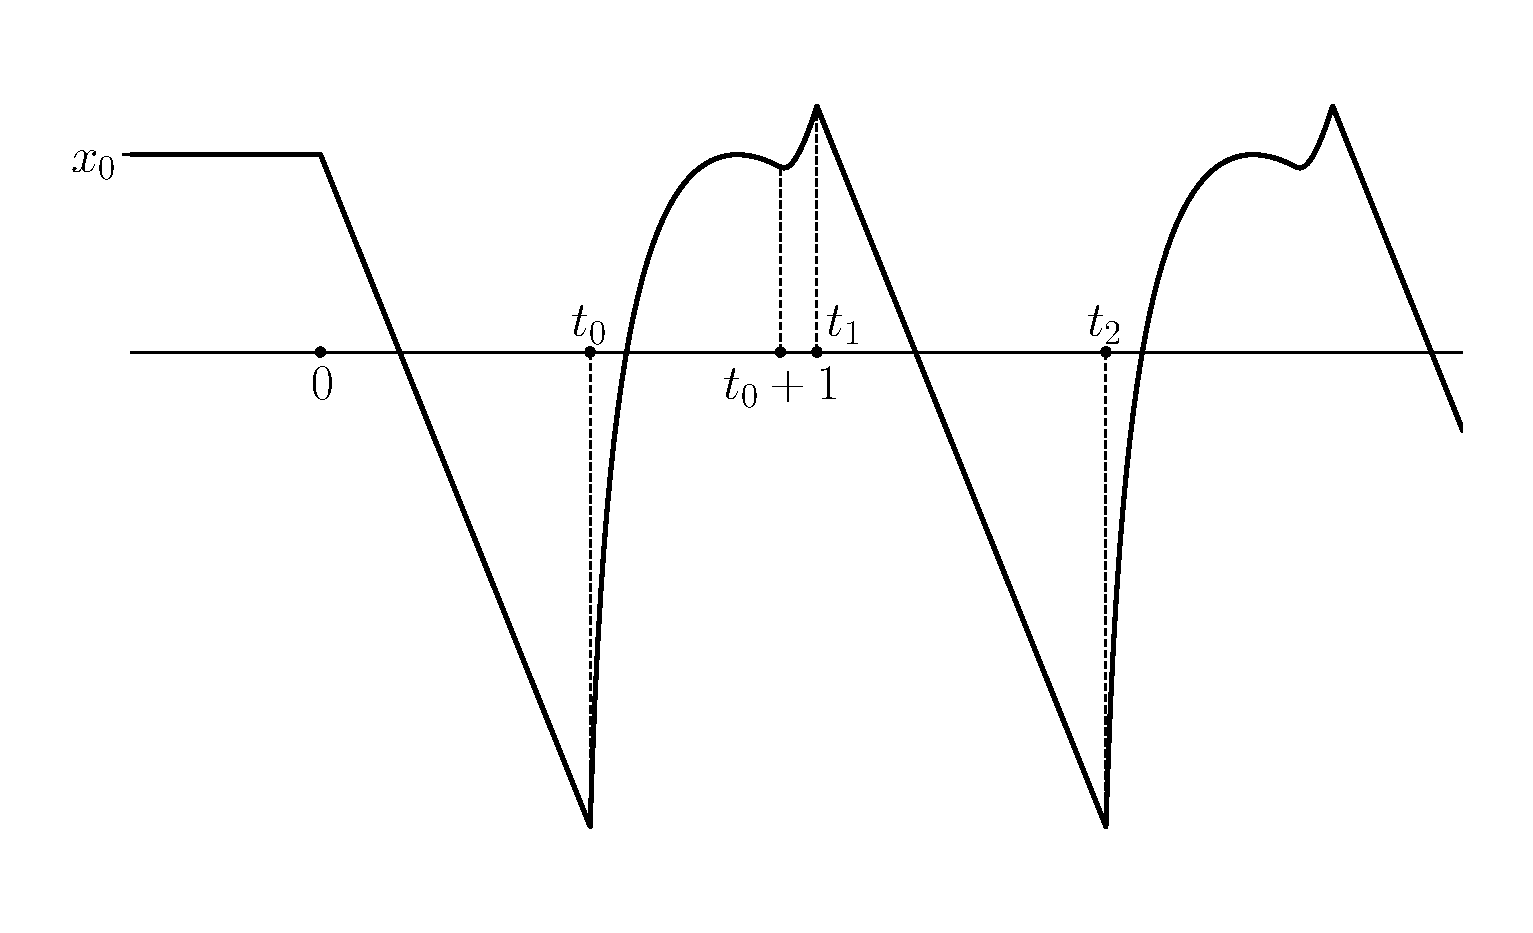
\includegraphics[width=0.7\textwidth]{x_star.eps}
  \captionof{figure}{Периодическое решение $x^{*}(t)$ уравнения \eqref{eq:MG_rele}.}
  \label{fig:x_star}
\end{figure}


\subsection{Доказательство теоремы о решении релейного уравнения}

Решение уравнения \eqref{eq:MG_rele} строится методом шагов.

Если $t \in [0, 1]$, то $x(t - 1) = \phi(t - 1) > 0$, следовательно $x(t)$ отыскивается из начальной задачи Коши
\begin{equation}
    \dot{x} = -\beta, \quad x|_{t = 0} = x_0,
\end{equation}
откуда $x(t) = x_0 - \beta t$. Аналитический вид решения сохраняется до точки $t_0$, поскольку в этой точке величина $x(t - 1)$ меняет знак.

На промежутке $t \in [t_0, t_0 + 1]$ величина $x(t - 1)$ отрицательна, поэтому решение отыскивается из задачи Коши

\begin{equation}
    \dot{x} = -\beta + \alpha\exp(x_0 - \beta(t - 1) - x), \quad x|_{t = t_0} = -\beta,
\end{equation}
откуда находим
\begin{equation}
    x(t) = x_0-\beta t +\ln(\alpha e^{\beta}(t-t_0)+1).
\end{equation}

Следующее изменение аналитического вида решения происходит либо при $t = t_0 + 2$ (в этот момент аргумент функции $x(t - 1)$ выходит из отрезка $[t_0, t_0 + 1]$), либо в точке, где $x(t - 1) = 0$, и величина $x(t - 1)$ второй раз меняет знак.

Проверим, что при ограничении \eqref{eq:cond_alpha1} выполнен второй случай, т.е. корень уравнения
\begin{equation}
\label{eq:t1_eq}
    x_0-\beta (t - 1) +\ln(\alpha e^{\beta}(t - t_0 - 1) + 1) = 0
\end{equation}
существует и лежит на промежутке $(t_0 + 1, t_0 + 2)$.

В \eqref{eq:t1_eq} обозначим $s = t - t_0$ и заменим $x_0 = \beta(t_0 - 1)$, получим
$$-\beta s + \ln(\alpha e^{\beta} (s - 1) + 1) = 0$$
%
или, эквивалентно,
%
\begin{equation}
\label{eq:t1_eq2}
e^{\beta s} - \alpha e^{\beta} (s - 1) - 1 = 0.
\end{equation}
Нужно показать, что при условии \eqref{eq:cond_alpha1} существует корень этого уравнения на промежутке $(1, 2)$.

Обозначим левую часть равенства \eqref{eq:t1_eq2} как $F(s) = e^{\beta s} - \alpha e^{\beta} (s - 1) - 1$. Исследуем функцию $F$:
%
\[
F'(s) = \beta e^{\beta s} - \alpha e^{\beta}, \quad F''(s) = \beta^2 e^{\beta s}.
\]
%
Поскольку $F''(s) > 0$, функция $F$ выпукла. Найдём точку минимума $s_{\min}$ из уравнения $F'(s) = 0$.
\[
\beta e^{\beta s} - \alpha e^{\beta} = 0 \Leftrightarrow s = 1 + \frac{1}{\beta}\ln\frac{\alpha}{\beta}.
\]
%
Поскольку при $\alpha > \beta$ верно $s_{\min} > 1$ и $F(1) = e^{\beta} - 1 > 0$, корень $s = s_* > 1$ существует тогда и только тогда, когда $F(s_{\min}) \leqslant 0$. Выразим $\alpha$ из этого условия.
%
\[
F(s_{\min}) = \frac{\alpha}{\beta}e^{\beta} - \frac{\alpha}{\beta}e^\beta\ln\frac{\alpha}{\beta} - 1 \leq 0 \Leftrightarrow \frac{\alpha}{\beta}e^{\beta}\left(1 + \ln\frac{\beta}{\alpha}\right) < 1.
\]

% Обозначим левую часть равенства \eqref{eq:t1_eq2} как $F(s)$; $F''(s) > 0$, поэтому $F(s)$ выпукла. Минимум $F(s)$ достигается в точке $s_{\min} = 1 + \frac{1}{\beta}\ln\frac{\alpha}{\beta}$. Поскольку $s_{\min} > 1$ и $F(1) = e^{\beta} - 1 > 0$, корень $s = s_* > 1$ существует тогда и только тогда, когда $F(s_{\min}) \leqslant 0$; это эквивалентно условию
% $$\alpha \geqslant \dfrac{-\beta e^{-\beta}}{W(-e^{-\beta - 1})}.$$

Условие $s_* < 2$ выполняется, если $F(2) < 0$ или $s_{\min} < 2$, что эквивалентно (в первом случае) $\alpha > e^{\beta} - e^{-\beta}$ или (во втором случае) $\alpha < \beta e^{\beta}$.

Совокупность приведённых условий (с точностью до замены нестрогих неравенств на строгие) эквивалентна \eqref{eq:cond_alpha1}, что показывает следующая лемма.

\begin{lemma}
\label{lm:parameter_constraints:ch1}
Совокупность неравенств 
\[
\begin{cases}
\left[
\begin{array}{ll}
	\alpha > e^{\beta} - e^{-\beta},\\
    \alpha < \beta e^{\beta},
\end{array}
\right.\\
\frac{\alpha}{\beta}e^{\beta}\left(1 + \ln\frac{\beta}{\alpha}\right) < 1
\end{cases}
\]
эквивалентна условиям \eqref{eq:cond_alpha1}.
\end{lemma}
\begin{proof}
Элементарными преобразованиями получаем: 
\[
e^{\beta} - e^{-\beta} = \beta e^{\beta} \Leftrightarrow (2\beta - 2) e^{2\beta - 2} = -2e^{-2}.
\]
Для отображения $t \mapsto te^t$ каждая точка из интервала $(-1, 0)$ имеет ровно два прообраза, следовательно, возможны две ситуации: $2\beta - 2 = -2$, откуда $\beta = 0$, и $2\beta - 2 = W(-2e^{-2})$, откуда $\beta = \tilde{\beta}$.

Также заметим, что $(e^{\beta} - e^{-\beta})'|_{\beta = 0} > (\beta e^{\beta})'|_{\beta = 0}$, поэтому на промежутке $(0, \tilde{\beta})$ верно неравенство $e^{\beta} - e^{-\beta} > \beta e^{\beta}$. На промежутке $(\tilde{\beta}, +\infty)$ верно обратное неравенство из асимптотических соображений при $\beta \to +\infty$.

Теперь явно выразим $\alpha$ из третьего неравенства в условии леммы.
\begin{equation*}
\frac{\alpha}{\beta}e^{\beta}\left(\ln\frac{\beta}{\alpha} + 1\right) < 1\ \Leftrightarrow\ 1 + \ln\dfrac{\beta}{\alpha} < \dfrac{\beta e^{-\beta}}{\alpha}.
\end{equation*}

Возьмём экспоненту от обеих частей:
\begin{equation*}
\dfrac{e\beta}{\alpha} < \exp\dfrac{\beta e^{-\beta}}{\alpha}\ \Leftrightarrow\ \dfrac{-\beta e^{-\beta}}{\alpha}\exp \dfrac{-\beta e^{-\beta}}{\alpha} > -e^{-\beta - 1}\ \Leftrightarrow
\end{equation*}

\begin{align}
\label{eq:step3_cond1_expanded:ch1}
\left[
\begin{array}{ll}
    -\frac{\beta e^{-\beta}}{\alpha} > W(-e^{-\beta - 1}),\\
    -\frac{\beta e^{-\beta}}{\alpha} < W_{-1}(-e^{-\beta - 1}).
\end{array}
\right.
\end{align}
%
где $W_{-1}(x)$ --- ветвь функции Ламберта, принимающая значения из промежутка $(-\infty; -1]$.

Однако, второе неравенство соответствует случаю $\dfrac{-\beta e^{-\beta}}{\alpha} < -1$, поскольку $W_{-1}(x) < -1$. Тогда
\[
\alpha < \beta e^{-\beta} < \beta,
\]
что противоречит условию $\alpha > \beta$.

Значит, совокупность неравенств \eqref{eq:step3_cond1_expanded:ch1} заменяется на единственное неравенство
\[
    -\frac{\beta e^{-\beta}}{\alpha} > W(-e^{-\beta - 1}) \Leftrightarrow \alpha > -\dfrac{\beta e^{\beta}}{W(-e^{-\beta - 1})}.
\]
%
Знак неравенства меняется, поскольку $W(-e^{-\beta - 1}) < 0$.

Докажем, что $-\dfrac{\beta e^{-\beta}}{W(-e^{-\beta - 1})} > \beta e^{\beta}$ тогда и только тогда, когда $0 < \beta < \tilde{\beta}$.
%
\[
-\dfrac{\beta e^{\beta}}{W(-e^{-\beta - 1})} > \beta e^{\beta} \Leftrightarrow W(-e^{-\beta - 1}) > -e^{-2\beta} \Leftrightarrow -e^{-\beta - 1} > -e^{-2\beta} \exp(-e^{-2\beta}) \Leftrightarrow
\]
%
\[
\Leftrightarrow e^{\beta - 1} < \exp(-e^{-2\beta}) \Leftrightarrow \beta - 1 < -e^{-2\beta} \Leftrightarrow \beta e^{\beta} < e^{\beta} - e^{-\beta}.
\]
Последнее неравенство верно при $0 < \beta < \tilde{\beta}$, как было доказано выше.

Докажем, что $-\dfrac{\beta e^{-\beta}}{W(-e^{-\beta - 1})} \leqslant e^{\beta} - e^{-\beta}$.

%% !!TODO: завершить доказательство!
\textbf{Здесь будет завершение доказательства. Оно есть во второй части в более общем случае, может можно сослаться или привести в виде леммы здесь.}

\end{proof}

На отрезке $t \in [t_0 + 1, t_1]$ решение отыскивается из задачи Коши 
%
\begin{multline}
    \dot{x} = -\beta + \alpha\exp\bigg(x_0 - \beta(t - 1) + \ln(\alpha e^{\beta}(t - t_0 - 1) + 1) - x\bigg),\\
    x|_{t = t_0 + 1} = x_0 - \beta (t_0 + 1) +\ln(\alpha e^{\beta} + 1),
\end{multline}
%
откуда находим
\begin{equation}
    x(t) = x_0-\beta t+\ln\left(\frac{\alpha^2}{2}e^{2\beta}(t-t_0-1)^2+\alpha e^{\beta}(t-t_0)+1\right).
\end{equation}
%
При $t > t_1$ величина $x(t - 1)$ становится положительной, поэтому уравнение \eqref{eq:MG_rele} вновь принимает вид $\dot{x} = -\beta$. Пусть $t_2$ --- следующий корень уравнения $x(t - 1) = 0$, а именно
\begin{equation}
\label{eq:t2}
t_2 = 1 + \dfrac{1}{\beta}\ln\left(\frac{\alpha^2}{2}e^{2\beta}(t-t_0-1)^2+\alpha e^{\beta}(t-t_0)+1\right).
\end{equation}

С учётом начальных условий в точке $t_1$, на промежутке $[t_1, t_2]$
\begin{equation}
\label{eq:sol_rele_3}
    x(t) = x_0-\beta t+\ln\left(\frac{\alpha^2}{2}e^{2\beta}(t_1-t_0-1)^2+\alpha e^{\beta}(t_1-t_0)+1\right).
\end{equation}

Отбросим в \eqref{eq:sol_rele_3} квадратичное слагаемое, получим выпуклую вверх функцию $\tilde{x}(t) = -\beta(t - t_0 + 1) + \ln(\alpha e^{\beta} (t - t_0) + 1)$, равную нулю в точке $t_1 - 1$. Тогда $\tilde{x}(t) > 0$ на промежутке $(t_1 - 1, t_1]$, если $\tilde{x}(t_1) > 0$. Выражая из этого неравенства $\alpha$, с учётом $x(t) \geqslant \tilde{x}(t)$ получим условие \eqref{eq:cond_alpha2}.

Пусть $t_2$ --- корень уравнения $x(t - 1) = 0$, больший $t_1$. Поскольку $x(t) > 0$ на промежутке длины не меньше единицы, последующие шаги построения решения будут совпадать с приведёнными выше, и решение $x(t)$ будет периодическим с периодом $T = t_2 - t_0$. Подставляя соответствующие значения из \eqref{eq:t0:ch1} и \eqref{eq:t2}, получаем явное значение периода \eqref{eq:T}.

% Отметим, что при $\alpha > \exp(\beta + e^{-\beta})$ условия теоремы выполняются (в этом можно убедиться явной проверкой условий).
% Расписать подробнее

\subsection{Явные ограничения на параметры уравнения}

Одновременное выполнение условий \eqref{eq:cond_alpha1} и \eqref{eq:cond_alpha2} затруднительно для проверки. Сформулируем достаточное условие, позволяющее легко находить подходящие наборы параметров $\alpha$ и $\beta$.

\begin{theorem}
Пусть параметры $\alpha$, $\beta$ таковы, что $\beta > 0$, $\alpha > \exp(\beta + e^{-\beta})$. Тогда $\alpha$ и $\beta$ удовлетворяют условиям \eqref{eq:cond_alpha1} и \eqref{eq:cond_alpha2}.
\end{theorem}
\begin{proof}
	Поскольку, очевидно, $\exp(\beta + e^{-\beta}) > e^{\beta} - e^{-\beta}$, условие \eqref{eq:cond_alpha1} выполнено.	
	
	%% !!TODO: завершить доказательство!
	\textbf{Здесь будет завершение доказательства. Оно есть во второй части в более общем случае, может можно сослаться или привести в виде леммы здесь.}
	
	
\end{proof}

%%%%%%
%%% ОСНОВНОЙ РАЗДЕЛ ПРО АСИМПТОТИКИ
%%%%%%
\section{Асимптотика уравнения Мэки--Гласса}


%% !!TODO: Здесь пока нет единтвенности. Для доказательства единственности надо написать производную Фреше.
\begin{theorem}
    \label{thm:existence}
Пусть параметры $\alpha > \beta > 0$ удовлетворяют условиям \eqref{eq:cond_alpha1}, \eqref{eq:cond_alpha2}. Тогда существуют такие значения параметров $x_0, p, q$ и такое достаточно большое $\gamma_0$, что при всех $\gamma > \gamma_0$ уравнение \eqref{eq:MG_x} с начальной функцией из множества \eqref{eq:init_set} обладает периодическим решением $x^*_\gamma(t)$ периода $T_\gamma$, которое удовлетворяет предельным равенствам 
\begin{equation}
\label{eq:lim_x*}
	\lim_{\gamma\to+\infty}\max_{0\leqslant t\leqslant T_\gamma}|x_{\gamma}^*(t)-x^*(t)|=0,\quad \lim_{\gamma\to+\infty}T_{\gamma} = T.
\end{equation}
\end{theorem}

\subsection{Общая схема доказательства}
Будем последовательно находить асимптотические формулы решения $x_{\gamma}^*(t)$ уравнения \eqref{eq:MG_x} методом шагов, опираясь на решение $x^*(t)$ релейного уравнения \eqref{eq:MG_rele}. Техника построения асимптотики сходна с описанной в работах \cite{Kolesov2010, Glyzin2013}.

Назовем \textit{точкой излома} функции $x^*(t)$ точку, в которой она имеет разные односторонние производные. Точки излома следует искать среди точек, в которых функция $x^*(t)$ меняет аналитический вид, то есть среди точек $t_0$, $t_0+1$, $t_1$. Однако, в точке $t_0+1$ производные справа и слева совпадают и равны $-\beta+\frac{\alpha e^{\beta}}{\alpha e^{\beta}+1}$, то есть $t_0+1$ не является точкой излома функции $x^*(t)$. Производные в точке $t_0$ справа и слева равны соответственно $-\beta$ и $-\beta+\alpha e^\beta$, в точке $t_1$ они равны $$-\beta+\frac{\alpha^2e^{2\beta}(t_1-t_0-1)+\alpha e^\beta}{\frac{\alpha^2}{2}e^{2\beta}(t_1-t_0-1)^2+\alpha e^{\beta}(t_1-t_0)+1}$$ слева и $-\beta$ справа. 
Таким образом, функция $x^*(t)$ имеет две точки излома: $t_0$ и $t_1$.

Зафиксируем параметр $\nu\in(\frac{1}{2}, 1)$ и введем малый параметр $\sigma$, который следующим образом связан с большим параметром $\gamma$:  
%
\[\sigma=\gamma^{-\nu}.\]
%
Параметр $\sigma$ имеет смысл радиуса малой окрестности точки излома.

На отрезках 
$[0,t_0-\sigma],$ 
$[t_0+\sigma, t_0+1-\sigma],$ 
$[t_0+1-\sigma,t_0+1+\sigma],$ 
$[t_0+1+\sigma,t_1-\sigma],$ 
$[t_1+\sigma,t_2-\sigma]$ 
будем искать решение в виде
%
\begin{equation}
    \label{eq:x*gamma_1}
    x^*_\gamma(t) = x^*(t) + \Delta
\end{equation}
и доказывать малость остатка $\Delta$. Для этого найдем задачу Коши, которой удовлетворяет остаток $\Delta$. С этой целью подставим \eqref{eq:x*gamma_1} в \eqref{eq:MG_x}, в результате чего получим уравнение
%
\begin{equation*}
    \dot{\Delta} = -\beta + \frac{\alpha\exp(x_{\gamma}^*(t - 1) - x^*(t))}{1 + \exp(\gamma x_{\gamma}^*(t - 1))}e^{-\Delta}-\dot{x}^*.
\end{equation*}
%
Обозначим начало рассматриваемого отрезка через $\tilde{t}$, а значение функции $\Delta$ в этой точке --- через $\tilde{\Delta}$. Для того чтобы найти начальное значение, приравняем значение в точке $\tilde{t}$ функции $x_{\gamma}^*(t)$ на предыдущем и текущем шагах:
%
\[x_{\gamma}^*(\tilde{t}-0)=x^*(\tilde{t}+0)+\Delta|_{t=\tilde{t}}.\]
%
Таким образом, $\Delta$ удовлетворяет задаче Коши
\begin{equation}
        \label{eq:task_DeltaAB}
        \dot{\Delta}=A e^{-\Delta} + B,\quad \Delta|_{t=\tilde{t}}=\tilde{\Delta},
\end{equation}
%
\begin{equation}
    \label{AB_eq:x*gamma_1}
\text{где } A = \frac{\alpha\exp(x_{\gamma}^*(t - 1) - x^*(t))}{1+\exp(\gamma x_{\gamma}^*(t - 1))},\, 
B = -\beta-\dot{x}^*,\, 
\tilde{\Delta}=x_{\gamma}^*(\tilde{t} - 0) - x^*(\tilde{t} + 0).
\end{equation}

На отрезках $[t_i - \sigma, t_i + \sigma],$ $i=0, 1,$ будем предполагать, что решение имеет вид
%
\begin{equation}
    \label{eq:x*gamma_2}
    x^*_\gamma(t)=x^*(t_i)+\frac{1}{\gamma}w_i(\tau)|_{\tau=(t-t_i)\gamma}+\Delta.
\end{equation}
%
Здесь $w_i(\tau)$ --- известные, специальным образом выбранные нами функции. Подробнее о них будет написано в следующем пункте. Параметр $\Delta$ --- предстоящий определению остаток, малость которого требуется доказать. Для определения задачи Коши, которой он удовлетворяет, подставим \eqref{eq:x*gamma_2} в \eqref{eq:MG_x} и найдем начальное значение. Получим задачу \eqref{eq:task_DeltaAB} при
\begin{equation}
    \label{AB_eq:x*gamma_2}
    A=\frac{\alpha\exp\big(x_{\gamma}^*(t-1)-x^*(t_i)-\frac{1}{\gamma}w_i(\tau)|_{\tau=(t-t_i)\gamma}\big)}{1+\exp(\gamma x_{\gamma}^*(t-1))},
    \,
    B=-\beta-\frac{dw_i}{d\tau}\Big|_{\tau=(t-t_i)\gamma},
\end{equation}
%
\begin{equation}\label{tilde_eq:x*gamma_2}
    \tilde{t} = t_i - \sigma = t_i - \gamma^{-\nu},\quad \tilde{\Delta}=x_{\gamma}^*(\tilde{t} - 0) - x^*(t_i) -\frac{1}{\gamma} w_i(\tau)|_{\tau = -\gamma^{1 - \nu}}.
\end{equation}
%% !!DONE: проверено.

Получаем, что на каждом из рассматриваемых отрезков, остаток $\Delta$ находится из задачи Коши \eqref{eq:task_DeltaAB}. Докажем вспомогательное утверждение.

\begin{lemma}\label{lm:DeltaAB}
Пусть $\tilde{t} \geqslant 0$, $\tilde{\Delta}$ --- известные вещественные числа, $A = A(t),$ $B = B(t)$ --- непрерывные при $t \geq \tilde{t}$ функции, $A(t) > 0$. Тогда решение задачи Коши \eqref{eq:task_DeltaAB} выражается формулой
	\begin{equation}\label{sol_DeltaAB}
	\Delta = J + \ln\Big(1 + \int\limits_{\tilde{t}}^{t} A(s) e^{-J}\,ds \Big),
	\text{ где } J = \tilde{\Delta} + \int\limits_{\tilde{t}}^{t} B(s)\,ds.
	\end{equation}
\end{lemma}
\begin{proof}
    Замена $e^{\Delta}=\theta$ преобразует задачу \eqref{eq:task_DeltaAB} к виду
	%
    \begin{equation}\label{task_theta}
		\dot{\theta}=A+B\theta,\quad\theta|_{t=\tilde{t}}=e^{\tilde{\Delta}}.
    \end{equation}
	%
    Решение соответствующей однородной задачи $\dot{\theta}=B\theta$, $\theta|_{t=\tilde{t}}=e^{\tilde{\Delta}}$ --- это функция $\theta_*(t)=\exp(\tilde{\Delta}+\int\limits_{\tilde{t}}^{t}B(s)ds).$ Тогда решение задачи \eqref{task_theta} --- это $\theta=\theta_* y$, где $y$ удовлетворяет задаче $\dot{y} = A \theta^{-1}$, $y|_{t=\tilde{t}} = 1$. Отсюда $y = 1 + \int\limits_{\tilde{t}}^{t}A(s)\theta_*^{-1}ds$, следовательно $\theta=\theta_*(1+\int\limits_{\tilde{t}}^{t}A(s)\theta_*^{-1}ds)$.
    Тогда $\Delta=\ln\theta=\ln\theta_*+\ln(1+\int\limits_{\tilde{t}}^{t}A(s)\theta_*^{-1}ds),$ откуда следует формула \eqref{sol_DeltaAB}.
\end{proof}
%%!! DONE: проверено.

Из леммы \eqref{lm:DeltaAB} и формул \eqref{AB_eq:x*gamma_1}, \eqref{AB_eq:x*gamma_2}, \eqref{tilde_eq:x*gamma_2} получаем следствия.
\begin{corollary}\label{corol_Delta_long}
На отрезках $[0, t_0-\sigma],$ $[t_0+\sigma, t_0+1-\sigma],$ $[t_0+1-\sigma, t_0+1+\sigma],$ $[t_0+1+\sigma, t_1-\sigma],$ $[t_1+\sigma,t_2-\sigma],$ где решение имеет вид \eqref{eq:x*gamma_1}, остаток $\Delta$ определяется формулой
\begin{equation}
    \label{Delta}
    \Delta = J + \ln(1 + I),
\end{equation}
где 
\begin{equation}
    \label{I_long}
    I = \int\limits_{\tilde{t}}^{t}\frac{\alpha\exp(x_{\gamma}^*(s-1)+\beta(s-\tilde{t})-x_{\gamma}^*(\tilde{t}))}{1 + \exp(\gamma x_{\gamma}^*(s-1))} ds,
\end{equation}
%
\begin{equation}\label{eq:J_long}
    J = x_{\gamma}^*(\tilde{t}) - x^*(t) - \beta(t - \tilde{t}),
\end{equation}
%
$\tilde{t}$ --- начальная точка рассматриваемого отрезка.
\end{corollary}
%
\begin{proof}
	Подставим в формулу \eqref{sol_DeltaAB} значения $A$ и $B$ из \eqref{AB_eq:x*gamma_1}. Получим $\Delta = J + \ln(1 + I)$, где
\begin{multline*}
	J = \tilde{\Delta} + \int\limits_{\tilde{t}}^{t}(-\beta - \dot{x}^*(s))ds = x_{\gamma}^*(\tilde{t}) - x^*(\tilde{t}) - \beta(t - \tilde{t}) - x^*(t) + x^*(\tilde{t}) =\\= x_{\gamma}^*(\tilde{t}) - x^*(t) - \beta(t - \tilde{t}),
\end{multline*}
\[
	I = \int\limits_{\tilde{t}}^{t} A e^{-J} \, ds = \int\limits_{\tilde{t}}^{t}\frac{\alpha\exp(x_{\gamma}^*(s-1)+\beta(s-\tilde{t})-x_{\gamma}^*(\tilde{t}))}{1 + \exp(\gamma x_{\gamma}^*(s-1))} ds.
\]
\end{proof}
%
\begin{corollary}\label{corol_Delta_short}
На отрезках $[t_i-\sigma,t_i+\sigma]$, $i=0, 1$, где решение имеет вид \eqref{eq:x*gamma_2}, остаток $\Delta$ определяется формулой \eqref{Delta} при
 \begin{equation}
    \label{I_point}
   I=\int\limits_{t_i-\sigma}^{t}\frac{\alpha\exp\big(x_{\gamma}^*(s-1)+\beta(s-t_i+\sigma)-x_{\gamma}^*(t_i-\sigma)\big)}{1+\exp(\gamma x_{\gamma}^*(s-1))}ds,
\end{equation}
%
\begin{equation}
    \label{J_point}
    J=x_{\gamma}^*(t_i - \sigma) - x^*(t_i) - \beta(t-t_i+\sigma) - \frac{1}{\gamma} w_i(\tau)|_{\tau=(t-t_i)\gamma}.
\end{equation}
\end{corollary}
%
\begin{proof}
	Выражая $\tilde{\Delta} = \Delta|_{t = t_i - \sigma}$ из \eqref{eq:x*gamma_2}, получаем
\[
	\tilde{\Delta} = x^*_{\gamma}(t_i - \sigma) - x^*(t_i) - \frac{1}{\gamma} w_i(\tau)|_{\tau = -\gamma^{1-\nu}}.
\]
Пусть $\tilde{t} = t_i - \sigma$. Учитывая $\frac{d}{d\tau} w_i(\tau)|_{\tau = \gamma(t - t_i)} = \frac{d}{dt} \left(\frac{1}{\gamma}w_i(\tau)\right)\big|_{\tau = \gamma(t - t_i)}$, в формуле \eqref{sol_DeltaAB} получаем
\begin{multline*}
	J = \tilde{\Delta} + \int\limits_{\tilde{t}}^{t} B(s)\,ds = \tilde{\Delta} + \int\limits_{\tilde{t}}^{t} -\beta - \frac{d}{ds} \left(\frac{1}{\gamma}w_i(\tau)\right)\big|_{\tau = \gamma(s - t_i)} \,ds =\\= x^*_{\gamma}(t_i - \sigma) - x^*(t_i) - \frac{1}{\gamma} w_i(\tau)|_{\tau = -\gamma^{1-\nu}} - \frac{1}{\gamma}w_i(\tau)|_{\tau = \gamma(t - t_i)} + \frac{1}{\gamma}w_i(\tau)_{\tau = -\gamma^{1 - \nu}} = \\
	= x^*_{\gamma}(t_i - \sigma) - x^*(t_i) - \beta(t - t_i - \sigma) - \frac{1}{\gamma} w_i(\tau)|_{\tau = \gamma(t - t_i)}.
\end{multline*}
%
По лемме \ref{lm:DeltaAB} получаем, что остаток имеет вид $\Delta = J + \ln(1 + I)$, где 
\[
I = \int\limits_{\tilde{t}}^{t}A(s) e^{-J} ds = \int\limits_{t_i-\sigma}^{t}\frac{\alpha\exp\big(x_{\gamma}^*(s-1)+\beta(s-t_i+\sigma)-x_{\gamma}^*(t_i-\sigma)\big)}{1+\exp(\gamma x_{\gamma}^*(s-1))}ds.
\]
\end{proof}
%% !!DONE: проверено.
%% !!TODO: добавить развёрнутые выкладки.
%
Отметим, что $x_{\gamma}^*(\tilde{t})$ и $x_{\gamma}^*(t_i-\sigma)$ в следствиях \ref{corol_Delta_long} и \ref{corol_Delta_short} определяются формулами, полученными на предыдущих шагах.

\subsection{Вспомогательные асимптотические соотношения}

В дальнейшем мы будем пользоваться следующими асимптотическими соотношениями:
\begin{equation}
\label{eq:exp_const}
	e^{\epsilon} = 1 + O(\epsilon) \text{ при } \epsilon \to 0;
\end{equation}
\begin{equation}
\label{eq:exp_linear}
	e^{\epsilon} = 1 + \epsilon + O(\epsilon^2) \text{ при } \epsilon \to 0;
\end{equation}
\begin{equation}
\label{eq:asymp_frac}
	\frac{1}{1 + \varepsilon} = 1 + O(\varepsilon) \text{ при } \epsilon \to 0;
\end{equation}
\begin{equation}
\label{eq:exp_frac}
	\dfrac{1}{1 + e^{x + \epsilon}} = \frac{1}{1 + e^x} + O(\epsilon) \text{ при } \epsilon \to 0.
\end{equation}
\begin{equation}
\label{eq:ln_frac}
\ln(x + \epsilon) = \ln x + \frac{\epsilon}{x} + O(\epsilon^2) \text{ при } \epsilon \to 0.
\end{equation}

Соотношения \eqref{eq:exp_const}, \eqref{eq:exp_linear}, \eqref{eq:asymp_frac} очевидны.

Соотношение \eqref{eq:exp_frac} верно и в случае, когда $x$ зависит от $\epsilon$. Действительно,
%
\[
\dfrac{1}{1 + e^x} - \dfrac{1}{1 + e^{x + \epsilon}} = \dfrac{e^x}{(1 + e^x)(1 + e^{x + \epsilon})} \cdot (e^{\epsilon} - 1) = \dfrac{e^x}{(1 + e^x)(1 + e^{x + \epsilon})} \cdot O(\epsilon),
\]
где коэффициент при $O(\epsilon)$ меньше единицы.
%
Соотношение \eqref{eq:ln_frac} доказывается следующим образом:
\[
\ln(x + \epsilon) = \ln x + \ln(1 + \frac{\epsilon}{x}) = \ln x + \frac{\epsilon}{x} + O(\epsilon^2).
\]
Без дополнительных уточнений оно применимо лишь в случаях, когда $x > 0$ --- константа (не зависит от $\epsilon$).

\subsection{Асимптотическое поведение в окрестности точек излома}

Как было написано выше, для описания асимптотического поведения решения уравнения \eqref{eq:MG_x} в окрестности точек излома $t_i$ введем специальные функции $w_i(t)$. В общем случае их вид зависит от знака $\dot{x}(t_i - 1)$. Докажем утверждения о виде данных функций.

\begin{lemma}
\label{lm:w}
	Пусть $x^*(t_i - 1) = 0$, при $t \in [t_i - \sigma, t_i + \sigma]$ верны соотношения:
	\[ x^*_{\gamma}(t_i - \sigma) = x^*(t_i - \sigma) + O(\gamma^{-2\nu}), \quad x^*_{\gamma}(t - 1) = x^*(t - 1) + O(\gamma^{-2\nu}).\]
	Тогда решение на данном промежутке имеет вид \eqref{eq:x*gamma_2}, где
	\[
	w_i(\tau) = -\beta \tau - \dfrac{\alpha e^{-x^*(t_i)}}{\dot{x}^*(t_i - 1)} \ln\left(e^{-\dot{x}^*(t_i - 1)\tau} + 1\right) \quad \text{при} \quad \dot{x}^*(t_i - 1) > 0,
	\]
	\[
	w_i(\tau) = (-\beta + \alpha e^{-x^*(t_i)})\tau - \dfrac{\alpha e^{-x^*(t_i)}}{\dot{x}^*(t_i - 1)} \ln\left(e^{\dot{x}^*(t_i - 1)\tau} + 1\right) \quad \text{при} \quad \dot{x}^*(t_i - 1) < 0,
	\]
	\[
	\Delta = O(\gamma^{-2\nu}).
	\]
\end{lemma}
%
\begin{proof}
	По следствию \ref{corol_Delta_short}, остаток $\Delta$ имеет вид \eqref{Delta}, где $I$ и $J$ определяются формулами \eqref{I_point} и \eqref{J_point} соответственно.
	
	Оценим $I$.
	
	\begin{equation}
	\label{eq:I_point_estimate}
	I = \int\limits_{t_i - \sigma}^{t} \dfrac{\alpha \exp(x^*_{\gamma}(s - 1) + \beta(s - t_i + \sigma) - x^*_{\gamma}(t_i - \sigma))}{1 + \exp(\gamma x^*_{\gamma}(s - 1))}\, ds = \ldots
	\end{equation}
	
	Воспользуемся равенствами
	\[
	x^*(s - 1) = O(\sigma), \quad \beta(s - t_i + \sigma) = O(\sigma), \quad x^*(t_i - \sigma) = x^*(t_i) + O(\sigma),
	\]
	получим
	\[
	x^*_{\gamma}(s - 1) + \beta(s - t_i + \sigma) - x^*_{\gamma}(t_i - \sigma) = -x^*(t_i) + O(\sigma).
	\]
	Тогда числитель \eqref{eq:I_point_estimate} оценивается как
	\begin{multline*}
	\alpha \exp(x^*_{\gamma}(s - 1) + \beta(s - t_i + \sigma) - x^*_{\gamma}(t_i - \sigma)) = \alpha \exp(-x^*(t_i) + O(\sigma)) =\\= \alpha e^{-x^*(t_i)} \exp(O(\sigma)) = \alpha e^{-x^*(t_i)} (1 + O(\sigma)).
	\end{multline*}
	
	Преобразуем \eqref{eq:I_point_estimate} в сумму интегралов:
	\[
	\ldots = \int\limits_{t_i - \sigma}^{t} \dfrac{\alpha e^{-x^*(t_i)}}{1 + \exp(\gamma x^*_{\gamma}(s - 1))}\, ds + \int\limits_{t_i - \sigma}^{t} \dfrac{\alpha e^{-x^*(t_i)} O(\sigma)}{1 + \exp(\gamma x^*_{\gamma}(s - 1))} \, ds = \ldots
	\]
	
	Второй интеграл оценим как $O(\sigma^2) = O(\gamma^{-2\nu})$. Для оценки первого интеграла воспользуемся равенством
	\[
	x^*_{\gamma}(s - 1) = x^*(s - 1) + O(\gamma^{-2\nu}) = (s - t_i)\dot{x}^*(t_i - 1) + O(\gamma^{-2\nu}).
	\]
	Здесь мы пользуемся тем, что функция $x^*(t)$ разложима по Тейлору до слагаемого второго порядка, а также учитываем $x^*(t_i - 1) = 0$. % Она гладкая везде за исключением изломов.  
	Тогда 
	\[
	\exp(\gamma x^*_{\gamma}(s - 1)) = \exp(\gamma(s - t_i)\dot{x}^*(t_i - 1) + O(\gamma^{1 - 2\nu})).
	\]
	Из выбора $\nu$, $O(\gamma^{1 - 2\nu})$ мало. Применяя равенство \eqref{eq:exp_frac}, получаем следующую оценку.
	\begin{multline*}
	\dfrac{1}{1 + \exp(\gamma x^*_{\gamma}(s - 1))} = \dfrac{1}{1 + \exp(\gamma (s - t_i) \dot{x}^*(t_i - 1) + O(\gamma^{1 - 2\nu}))} =\\= \dfrac{1}{1 + \exp(\gamma(s - t_i)\dot{x}^*(t_i - 1))} + O(\gamma^{1 - 2\nu}).
	\end{multline*}
	Таким образом,
	\begin{multline*}
	\int\limits_{t_i - \sigma}^{t} \dfrac{\alpha e^{-x^*(t_i)} ds}{1 + \exp(\gamma x^*_{\gamma}(s - 1))} = \int\limits_{t_i - \sigma}^{t} \left(\dfrac{\alpha e^{-x^*(t_i)}}{1 + \exp(\gamma(s - t_i)\dot{x}^*(t_i - 1))} + O(\gamma^{1 - 2\nu})\right) ds =\\
	= \dfrac{\alpha e^{-x^*(t_i)}}{\gamma \dot{x}^*(t_i - 1)}\ln\left(1 + \exp(-\gamma(s - t_i)\dot{x}^*(t_i - 1))\right)\bigg\vert_{t_i - \sigma}^t + O(\gamma^{1 - 3\nu}) = \\
	= \dfrac{\alpha e^{-x^*(t_i)}}{\gamma \dot{x}^*(t_i - 1)}\ln\left(1 + \exp(-\gamma(t - t_i)\dot{x}^*(t_i - 1))\right) -\\- \dfrac{\alpha e^{-x^*(t_i)}}{\gamma \dot{x}^*(t_i - 1)}\ln\left(1 + \exp(\gamma^{1 - \nu}\dot{x}^*(t_i - 1))\right) + O(\gamma^{1 - 3\nu}).
	\end{multline*}
	Если $\dot{x}^*(t_i - 1) < 0$, второе слагаемое экспоненциально мало, и мы получаем оценку 
	\begin{equation}
	\label{eq:I_estimate_dotx_less_0}
	I = \dfrac{\alpha e^{-x^*(t_i)}}{\gamma \dot{x}^*(t_i - 1)}\ln\left(1 + \exp(-\gamma(t - t_i)\dot{x}^*(t_i - 1))\right) + O(\gamma^{1 - 3\nu}).
	\end{equation}
	Если $\dot{x}^*(t_i - 1) > 0$, 
	\begin{multline}
	\dfrac{\alpha e^{-x^*(t_i)}}{\gamma \dot{x}^*(t_i - 1)}\ln\left(1 + \exp(-\gamma(t - t_i)\dot{x}^*(t_i - 1))\right) -\\- \dfrac{\alpha e^{-x^*(t_i)}}{\gamma \dot{x}^*(t_i - 1)}\ln\left(1 + \exp(\gamma^{1 - \nu}\dot{x}^*(t_i - 1))\right) =\\
	= \dfrac{\alpha e^{-x^*(t_i)}}{\gamma \dot{x}^*(t_i - 1)}\ln\left(1 + \exp(\gamma(t - t_i)\dot{x}^*(t_i - 1))\right) - \alpha (t - t_i) e^{-x^*(t_i)} -\\- \dfrac{\alpha e^{-x^*(t_i)}}{\gamma \dot{x}^*(t_i - 1)}\ln\left(1 + \exp(-\gamma^{1 - \nu}\dot{x}^*(t_i - 1))\right) + \alpha \sigma e^{-x^*(t_i)}. 
	\end{multline}
	При $\dot{x}^*(t_i - 1) > 0$ третье слагаемое экспоненциально мало, и мы получаем следующую оценку.
	\begin{multline}
		\label{eq:I_estimate_dotx_greater_0}
		I = \dfrac{\alpha e^{-x^*(t_i)}}{\gamma \dot{x}^*(t_i - 1)}\ln\left(1 + \exp(\gamma(t - t_i)\dot{x}^*(t_i - 1))\right) -\\- \alpha (t - t_i - \sigma) e^{-x^*(t_i)} + O(\gamma^{1 - 3\nu}).
	\end{multline}
	
	Оценим $J$.
	
	При $\dot{x}^*(t_i - 1) < 0$ на промежутке $[t_i - \sigma, t_i]$ уравнение \eqref{eq:MG_rele} имеет вид $\dot{x} = -\beta$, следовательно, 
	\[
	\dot{x}_{\gamma}^*(t_i - \sigma) - x^*(t_i) = \dot{x}^*(t_i - \sigma) - x^*(t_i) + O(\gamma^{-2\nu}) = -\beta \sigma + O(\gamma^{-2\nu}).
	\]
	%
	Подставляя в \eqref{J_point} это равенство и функцию $w(\tau)$ из условия теоремы, получаем
	\begin{multline}
		\label{eq:J_estimate_dotx_less_0}
	J = -\beta \sigma + O(\gamma^{-2\nu}) + \beta (t - t_i) - \dfrac{\alpha e^{-x^*(t_i)}}{\gamma \dot{x}^*(t_i - 1)} \ln\left(e^{-\dot{x}^*(t_i - 1)\tau} + 1\right) - \beta(t - t_i - \sigma) =\\
	\\= -\dfrac{\alpha e^{-x^*(t_i)}}{\gamma \dot{x}^*(t_i - 1)} \ln\left(e^{-\dot{x}^*(t_i - 1)\tau} + 1\right) + O(\gamma^{-2\nu}).
	\end{multline}
	
	Заметим, что в обоих случаях $I = O(\gamma^{-\nu})$, тогда 
	\begin{equation}
	\label{eq:ln_1_plus_I}
	\ln(1 + I) = I + O(\gamma^{-2\nu}).
	\end{equation}
	
	Подставляя \eqref{eq:I_estimate_dotx_less_0} и \eqref{eq:J_estimate_dotx_less_0} в \eqref{Delta}, получаем
	\[
	\Delta = J + \ln(1 + I) = O(\gamma^{-2\nu}).
	\]
	
	При $\dot{x}^*(t_i - 1) < 0$ получаем
	\begin{multline}
	\label{eq:J_estimate_dotx_greater_0}
	J = x_{\gamma}^*(t_i - \sigma) - x^*(t_i) - (-\beta + \alpha e^{-x^*(t_i)})(t - t_i) +\\+ \dfrac{\alpha e^{-x^*(t_i)}}{\gamma \dot{x}^*(t_i - 1)} \ln\left(e^{\dot{x}^*(t_i - 1)\tau} + 1\right) - \beta(t - t_i + \sigma) =\\
	= x^*(t_i - \sigma) - x^*(t_i) - \alpha e^{-x^*(t_i)}(t - t_i) + \dfrac{\alpha e^{-x^*(t_i)}}{\gamma \dot{x}^*(t_i - 1)} \ln\left(e^{\dot{x}^*(t_i - 1)\tau} + 1\right) -\\- \beta\sigma + O(\gamma^{-2\nu}).
	\end{multline}
	
	Подставляя \eqref{eq:I_estimate_dotx_less_0} и \eqref{eq:J_estimate_dotx_less_0} в \eqref{Delta}, и пользуясь оценкой \eqref{eq:ln_1_plus_I}, получаем
	\[
	\Delta = x^*(t_i - \sigma) - x^*(t_i) - \beta \sigma - \alpha (t - t_i - \sigma) e^{-x^*(t_i)} + O(\gamma^{-2\nu}).
	\]
	С учётом 
	\[
	x^*(t_i - \sigma) - x^*(t_i) = -\sigma\dot{x}(t_i - 0) + O(\sigma^2),
	\]
	\[
	\dot{x}(t_i - 0) = \beta + \alpha e^{x^*(t_i - 1) - x^*(t_i)} = \beta + \alpha e^{-x^*(t_i)}
	\]
	получаем
	\[
	\Delta = O(\gamma^{-2\nu}).
	\]
\end{proof}

Сформулируем и докажем утверждение, описывающее асимптотическое поведение введенных функций $w_i(\tau)$ при $\tau\to-\infty$ и $\tau\to+\infty$.
%
\begin{lemma}\label{lm:lem_w_asymp} Верны следующие асимптотические равенства.

Если $\dot{x}(t_i - 1) < 0$,
\begin{equation}
	\label{eq:w0_asymp-}
	w_i(\tau) = -\beta \tau + O(\exp(-\dot{x}^*(t_i - 1) \tau)) \text{ при } \tau \to -\infty,
\end{equation}
\begin{equation}
	\label{eq:w0_asymp+}
	w_i(\tau) = (-\beta + \alpha e^{-x^*(t_i)})\tau + O(\exp(\dot{x}^*(t_i - 1) \tau)) \text{ при } \tau \to +\infty,
\end{equation}
	
Если $\dot{x}(t_i - 1) > 0$,
\begin{equation}
	\label{eq:w1_asymp-}
	w_i(\tau) = (-\beta + \alpha e^{-x^*(t_i)})\tau + O(\exp(\dot{x}^*(t_i - 1) \tau)) \text{ при } \tau \to -\infty,
\end{equation}
\begin{equation}
	\label{eq:w1_asymp+}
	w_i(\tau) = -\beta \tau + O(\exp(-\dot{x}^*(t_i - 1) \tau)) \text{ при } \tau \to +\infty.
\end{equation}
\end{lemma}
\begin{proof}
	При $\dot{x}(t_i - 1) < 0$ верна формула
	\[
	w_i(\tau) = -\beta \tau - \dfrac{\alpha e^{-x^*(t_i)}}{\dot{x}^*(t_i - 1)} \ln\left(e^{-\dot{x}^*(t_i - 1)\tau} + 1\right).
	\]
	
	При $\tau \to -\infty$,
	\[
	\ln\left(e^{-\dot{x}^*(t_i - 1)\tau} + 1\right) = O(\exp(-\dot{x}^*(t_i - 1)\tau)),
	\]
	 откуда следует \eqref{eq:w0_asymp-}.
	 
	При $\tau \to +\infty$,
	\begin{multline*}
	\dfrac{\alpha e^{-x^*(t_i)}}{\dot{x}^*(t_i - 1)} \ln\left(e^{-\dot{x}^*(t_i - 1)\tau} + 1\right) = -\dot{x}^*(t_i - 1)\tau)) = \alpha e^{-x^*(t_i)} \tau + \ln\left(e^{\dot{x}^*(t_i - 1)\tau} + 1\right) =\\
	= \alpha e^{-x^*(t_i)} \tau + O(\exp(\dot{x}^*(t_i - 1) \tau)),
	\end{multline*}
	откуда следует \eqref{eq:w0_asymp+}.
	
	Доказательство формул \eqref{eq:w1_asymp-} и \eqref{eq:w1_asymp+} производится аналогично.
\end{proof}

\begin{remark}
	Коэффициенты при $\tau$ в формулах \eqref{eq:w0_asymp-},\eqref{eq:w0_asymp+},\eqref{eq:w1_asymp-},\eqref{eq:w1_asymp+} совпадают с односторонними производными в точках $x^*(t_i)$ при $i = 0, 1$. 
\end{remark}

Подставляя соответствующие значения $x(t_i),$ $\dot{x}(t_i + 1)$ при $i = 0, 1,$ получаем
\begin{equation}
	\label{eq:w0}
	w_0(\tau)=-\beta \tau+\frac{\alpha e^\beta}{\beta}\ln(e^{\beta\tau}+1),
\end{equation}

\begin{multline}
	\label{eq:w1}
	w_1(\tau)=\left(-\beta + \frac{\alpha e^\beta(\alpha e^\beta(t_1-t_0-1)+1)}{\frac{\alpha^2}{2}e^{2\beta}(t_1-t_0-1)^2+\alpha e^{\beta}(t_1-t_0) + 1}\right)\tau -\\- \frac{\alpha e^\beta(\alpha e^\beta(t_1-t_0-1)+1)^2}{(-\beta(\alpha e^\beta(t_1-t_0-1)+1)+\alpha e^\beta)(\frac{\alpha^2}{2}e^{2\beta}(t_1-t_0-1)^2+\alpha e^{\beta}(t_1-t_0)+1))}\times
	\\ \times\ln\Bigg(\exp\Big(\beta\tau-\frac{\alpha e^\beta\tau}{\alpha e^\beta(t_1-t_0-1)+1}\Big)+1\Bigg).
\end{multline}

\subsection{Построение асимптотики}

Докажем следующую теорему об асимптотическом поведении решения уравнения \eqref{eq:MG_x}.

\begin{theorem}
\label{thm:th_asymp}
Пусть параметры $\alpha,$ $\beta$ удовлетворяют условиям теоремы \ref{thm:existence}, $\alpha > \beta e^{\beta}$, $\gamma \gg 1$, $\sigma = \gamma^{-\nu}$, $\nu \in (\frac{1}{2}, 1)$. Уравнение \eqref{eq:MG_x} с произвольной начальной функцией $\varphi$ из класса \eqref{eq:init_set} имеет решение $x_\gamma^*(t)$ с асимптотикой
\footnotesize
\begin{equation}
	\label{eq:sol_x*gamma}
	x^*_\gamma(t)= 
	\begin{cases}
		x_0 - \beta t + (\gamma^{-1} e^{-\beta \sigma \gamma}), & t\in[0, t_0 - \sigma],\\
		-\beta + \frac{1}{\gamma} w_0(\tau)|_{\tau=(t-t_0)\gamma} + O(\gamma^{-2\nu}), & t \in [t_0-\sigma,t_0+\sigma]\\
		x_0 - \beta t + \ln(\alpha e^{\beta}(t - t_0)+1) + O(\gamma^{-2\nu}) & t\in[t_0 + \sigma, t_0 + 1]\\
		x_0 - \beta t + \ln(\frac{\alpha^2}{2}e^{2 \beta}(t - t_0 - 1)^2 + \alpha e^{\beta}(t - t_0) + 1) + O(\gamma^{-2\nu}) & t \in [t_0 + 1, t_1 - \sigma]\\
		x_0 - \beta t_1 + \ln(\eta)+\frac{1}{\gamma} w_1(\tau)|_{\tau=(t - t_1)\gamma} + O(\gamma^{-2\nu}) & t\in[t_1 - \sigma, t_1  +\sigma]\\
		x_0 - \beta t + \ln(\eta) + O(\gamma^{-2\nu}) & t \in [t_1+\sigma, t_2-\sigma]
	\end{cases}
\end{equation}
\normalsize
где $\eta=\frac{\alpha^2}{2}e^{2\beta}(t_1 - t_0 - 1)^2 + \alpha e^{\beta}(t_1 - t_0) + 1$.
Асимптотические выражения написаны здесь в предположении $\gamma\to+\infty$.
Все остатки равномерны по $\varphi \in S$ и $t$ из соответствующих промежутков.
\end{theorem}

Для построения асимптотики функции $x_\gamma^*(t)$ последовательно рассмотрим семь отрезков:
$[0, t_0 - \sigma]$, 
$[t_0  -\sigma, t_0 + \sigma]$,
$[t_0 + \sigma, t_0 + 1 - \sigma]$,
$[t_0 + 1 - \sigma, t_0 + 1 + \sigma]$,
$[t_0 + 1 + \sigma, t_1 - \sigma]$,
$[t_1 - \sigma, t_1 + \sigma]$,
$[t_1 + \sigma, t_2 - \sigma]$.

\subsubsection{Первый шаг построения асимптотики}

Рассмотрим отрезок $[0, t_0 - \sigma]$. На этом отрезке будем искать решение в виде
%
\begin{equation}
	\label{eq:sol_1}
	x_\gamma^*(t) = x_0 - \beta t + \Delta_1,
\end{equation}
%
где $\Delta_1 = \Delta_1(t, \phi)$ --- остаток, порядок малости которого нужно установить. Докажем следующий факт.
%
\begin{lemma}
\label{lm:Delta1}
На отрезке $[0, t_0 - \sigma]$ функция $x_\gamma^*(t)$ описывается формулой \eqref{eq:sol_1}, причем
%
\[
\Delta_1 = O\left(\frac{1}{\gamma} e^{-\gamma^{1 - \nu}}\right) \text{ при } \gamma \to +\infty.
\]
\end{lemma}
\begin{proof}
Подставим \eqref{eq:sol_1} в \eqref{eq:MG_x}. Сначала рассмотрим отрезок $[0,1]$. Учитывая, что на этом отрезке $x(t-1) = \varphi(t-1)$ и $x_\gamma^*(0)=x_0 +\Delta|_{t=0}=x_0$, получаем следующую задачу Коши для нахождения $\Delta$: 
\begin{equation}
	\label{task_Delta1}
	\dot{\Delta}_1=\frac{\alpha \exp(\varphi(t-1)-x_0+\beta t-\Delta_1)}{1+\exp(\gamma\varphi(t-1))},\quad \Delta_1|_{t=0}=0.
\end{equation}

Дифференциальное уравнение \eqref{task_Delta1} --- уравнение с разделяющимися переменными. Домножим правую и левую части на экспоненту $e^{\Delta_1}$ и проинтегрируем:
%
\[
\int\limits_0^{\Delta_1} e^\Delta d\Delta=\int\limits_0^t \frac{\alpha \exp(\varphi(s-1) - x_0 + \beta s)}{1 + \exp(\gamma\varphi(s - 1))}ds.
\]
%
Интеграл слева равен $e^{\Delta_1} - 1$. Оценим интеграл в правой части.

Экспонента $e^{\beta s}$ в числителе под знаком интеграла ограничена, так как $s$ изменяется на конечном отрезке. Поскольку $\varphi\in S$, верно неравенство
%
\[
\frac{\exp\varphi(s - 1)}{1 + \exp(\gamma\varphi(s - 1))} \leqslant \frac{e^q}{1 + e^{\gamma p}}.
\]
Следовательно существует положительная константа $C$ (её точное значение неважно), такая что
\[
\int\limits_0^t\frac{\alpha\exp\varphi(s-1)-x_0+\beta s}{1+\exp(\gamma\varphi(s-1))}ds\leqslant\frac{C}{1+e^{\gamma p}}.
\]
%
Таким образом, 
\[
e^{\Delta_1}-1=O\Big(\frac{1}{1+e^{\gamma p}}\Big)=O(e^{-\gamma p}).
\]
Отсюда 
\[
\Delta_1=\ln(1+O(e^{-\gamma p}))=O(e^{-\gamma p}) \text{ при }t\in[0,1].
\]
Отметим, что полученная оценка равномерна по $t$ и $\varphi$.

Далее рассмотрим отрезок $[1, \tilde{t}],$ где $t = \min\{t_0 - \sigma, 2\}$. Здесь по доказанному выше $x_\gamma^*(t-1)=x_0-\beta (t-1)+O(e^{-p\gamma})=-\beta (t-t_0)+O(e^{-p\gamma})$.


Далее, рассмотрим отрезок $[1,\min\{t_0-\sigma,2\}]$. Здесь по доказанному выше $x_\gamma^*(t-1)=x_0-\beta (t-1)+O(e^{-p\gamma})=-\beta (t-t_0)+O(e^{-p\gamma})$. 

По следствию \eqref{corol_Delta_long}, на этом отрезке остаток имеет вид \eqref{Delta}. Оценим $J$ и $I$.
%
\[
J = x^*_{\gamma}(1) - x^*(t) - \beta (t - 1) = x_0 - \beta + O(e^{-p\gamma}) - (x_0 - \beta t) - \beta(t - 1) = O(e^{-p\gamma}).
\]
%
\[
I = \int\limits_{1}^{t}\frac{\alpha\exp(x_{\gamma}^*(s-1)+\beta(s-1)-x_{\gamma}^*(1))}{1 + \exp(\gamma x_{\gamma}^*(s-1))} ds.
\]
Заметим, что
\begin{multline*}
x_{\gamma}^*(s-1)+\beta(s-1)-x_{\gamma}^*(1) = x^*(s - 1) + O(e^{-p\gamma}) + \beta(s - 1) - x^*(1) + O(e^{-p\gamma}) =\\= x_0 - \beta(s - 1) + \beta(s - 1) - x_0 - \beta + O(e^{-p\gamma}) = \beta + O(e^{-p\gamma}),
\end{multline*}
\[
\gamma x^*_{\gamma}(s - 1) = \gamma (x^*(s - 1) + O(e^{-p\gamma}) = -\beta \gamma (s - t_0) + O(\gamma e^{-p\gamma}).
\]
Тогда 
\[
I = \int\limits_{1}^{t}\frac{\alpha\exp(\beta + O(e^{-p\gamma}))}{1 + \exp(-\beta \gamma (s - t_0) + O(\gamma e^{-p\gamma})} ds = \ldots
\]
Воспользуемся асимптотическими равенствами \eqref{eq:exp_const} и \eqref{eq:exp_frac}.
\begin{multline*}
\ldots = \alpha e^{\beta} \int\limits_{1}^{t}\left(\frac{1}{1 + \exp(-\beta \gamma (s - t_0))} + O(\gamma e^{-p\gamma})\right)(1 + O(e^{-p\gamma})) ds = \\
= \frac{\alpha e^{\beta}}{\beta \gamma} \left(\ln(1 + \exp(\beta \gamma (s - t_0)))\right)\bigg\vert_1^t + O(\gamma e^{-p\gamma}) = \\
= \frac{\alpha e^{\beta}}{\beta \gamma}  \big(\ln(1 + \exp(-\beta \gamma (t_0 - t))) - \ln(1 + \exp(-\beta \gamma (t_0 - 1)))\big) + O(\gamma e^{-p\gamma}) = \ldots 
% \\ O(\frac{1}{\gamma} e^{-\beta (t_0 - 2) \gamma}) + .
\end{multline*}
%
Если $t_0 - \sigma > 2$, то первый логарифм оценивается как $O(\exp(-\beta \gamma (t_0 - 2)))$; если $t_0 - \sigma \leq 2$, то $O(\exp(-\beta \gamma^{1 - \nu}))$, что асимптотически больше $O(\gamma e^{-p\gamma})$. Таким образом, получаем
\[
I = 
\begin{cases}
O(e^{-C \gamma}) & \text{ при } t_0 - \sigma > 2,\\
O(\frac{1}{\gamma} e^{-\beta \gamma^{1 - \nu}}) & \text{ при } t_0 - \sigma \leq 2,
\end{cases}
\]
где $C > 0$ --- некоторая константа, значение которой не важно.

Значит,
\begin{equation}
	\label{eq:Delta_step1}
\Delta = J + \ln(1 + I) = 
\begin{cases}
	O(e^{-C \gamma}) & \text{ при } t_0 - \sigma > 2,\\
	O(\frac{1}{\gamma} e^{-\beta \gamma^{1 - \nu}}) & \text{ при } t_0 - \sigma \leq 2.
\end{cases}
\end{equation}

Если $t_0 - \sigma > 2$, продолжим двигаться шагами длины $1$. Каждый раз остаток будет такого вида, как в \eqref{eq:Delta_step1} (вместо двойки будет натуральное число, соответствующее номеру шага длины $1$). В конце, когда дойдем до точки $t_0 - \sigma$, получим
%
\[
\Delta_1=O(\gamma^{-1} e^{-\beta\gamma^{1 - \nu}}).
\]
%
Лемма \ref{lm:Delta1} доказана.

\end{proof}

\subsubsection{Второй шаг построения асимптотики}
Очередной промежуток построения решения --- это $[0, t_0 - \sigma]$. Поскольку на отрезке $[0, t_0 - \sigma]$ доказана (даже более точная) оценка $x^*_\gamma(t) = x^*(t) + O(\gamma^{-2\nu})$, применима лемма \ref{lm:w} для случая $\dot{x}(t_i - 1) < 0$. Из неё следует, что при $t \in [t_0 - \sigma, t_0 + \sigma]$ верна оценка
\begin{equation}
	\label{eq:sol_2}
	x_{\gamma}^*(t) = x^*(t) + \frac{1}{\gamma} w_0(\tau)\bigg\vert_{\tau=(t - t_0)\gamma} + \Delta_2,
\end{equation}
где $\Delta_2 = O(\gamma^{-2\nu})$. Напомним, функция $w_0(\tau)$ в явном виде описана формулой \ref{eq:w0}.

\subsubsection{Третий шаг построения асимптотики}
Рассмотрим отрезок $[t_0 + \sigma, t_0 + 1 - \sigma]$. Здесь решение отыскивается в виде
\begin{equation}
	\label{eq:sol_3}
	x_\gamma^*(t) = x^*(t) + \Delta_3,
\end{equation}
где $x^*(t) = x_0 - \beta t +\ln(\alpha e^{\beta}(t - t_0)+1),$ $\Delta_3 = \Delta_3(t, \phi)$ --- очередной остаток, предстоящий определению. Докажем следующий факт.

\begin{lemma}
	\label{lm:Delta3}
	На отрезке $[t_0 + \sigma, t_0 + 1 - \sigma]$ функция $x_\gamma^*(t)$ описывается формулой \eqref{eq:sol_3}, причем
	\[
	\Delta_3 = O(\gamma^{-2\nu}) \text{ при } \gamma \to +\infty.
	\]
\end{lemma}
\begin{proof}
Применим следствие \ref{corol_Delta_long} при $\tilde{t} = t_0 + \sigma$. С учетом асимптотического поведения \eqref{eq:w0_asymp+} функции $w_0(\tau)$ верно
\begin{equation}
\label{eq:x_gamma_t0_sigma_step3}
	x_\gamma^*(t_0 + \sigma) = -\beta + \frac{1}{\gamma} w_0(\tau)|_{\tau=\gamma^{1 - \nu}} + O(\gamma^{-2\nu}) = -\beta + (-\beta + \alpha e^\beta)\sigma + O(\gamma^{-2\nu}).
\end{equation}

Подставим \eqref{eq:x_gamma_t0_sigma_step3} и явный вид $x^*(t)$ в формулу \eqref{eq:J_long}. Получаем:
\begin{multline}
	\label{eq:J_step3}
	J = x_\gamma^*(t_0 + \sigma) - x^*(t) - \beta(t - t_0 - \sigma) =\\
	= -\beta + (-\beta + \alpha e^\beta)\sigma + O(\gamma^{-2\nu}) - 
	(-\beta(t - t_0 + 1) + \ln(\alpha e^{\beta}(t - t_0))) - \beta (t - t_0 - \sigma) = \\
	 =\alpha e^\beta\sigma + O(\gamma^{-2\nu}) - \ln(\alpha e^{\beta}(t - t_0) + 1).
\end{multline}

Далее оценим значение $I$. Подставим
%
\begin{multline*}
x^*_{\gamma}(s - 1) + \beta (s - t_0 - \sigma) - x^*_{\gamma} (t_0 + \sigma) =\\
= x_0 - \beta(s - 1) + \beta(s - t_0 - \sigma) + \beta + (\beta - \alpha e^{\beta}) \sigma + O(\gamma^{-2\nu}) =\\
= \beta - \alpha e^{\beta} \sigma + O(\gamma^{-2\nu})
\end{multline*}
%
в формулу \eqref{I_long}. Получим:
\begin{multline*}
	I=\int\limits_{t_0+\sigma}^{t}\frac{\alpha\exp(x_\gamma^*(s-1)+\beta(s-t_0-\sigma)-x_\gamma^*(t_0+\sigma))}{1+\exp(\gamma x_\gamma^*(s-1))} ds =\\
	=\int\limits_{t_0+\sigma}^{t}\frac{\alpha e^{\beta}\exp(-\alpha e^\beta\sigma+O(\gamma^{-2\nu}))}{1+\exp( -\beta\gamma (s-1)+O(e^{-\beta\sigma\gamma}))} ds,
\end{multline*}
%
что, с учётом асимптотических равенств \eqref{eq:exp_linear} и \eqref{eq:exp_frac}, преобразуется к виду
\begin{multline*}
	I = \int\limits_{t_0 + \sigma}^{t}\Big(\frac{\alpha e^\beta}{1 + \exp(-\beta\gamma(s-t_0))} + O(\gamma e^{-\beta\sigma\gamma})\Big) \cdot \big(1-\alpha e^{\beta} \gamma^{-\nu} + O(\gamma^{-2\nu})\big)ds=\\
	\int\limits_{t_0+\sigma}^{t}\Big(\frac{\alpha e^\beta(1-\alpha e^{\beta}\sigma)}{1 + \exp(-\beta\gamma(s-t_0))} + O(\gamma^{-2\nu})\Big)ds=\\
	= \frac{\alpha e^{\beta}}{\beta\gamma}\big(\ln(e^{\beta\gamma(t - t_0)} + 1) - \ln(e^{\beta\gamma^{1-\nu}}+1)\big)(1-\alpha e^{\beta}\sigma)+O(\gamma^{-2\nu})=\\
	= \frac{\alpha e^{\beta}}{\beta\gamma}\big(\ln(e^{\beta\gamma(t-t_0)}(1 + e^{-\beta\gamma(t - t_0)})) - \ln(e^{\beta\gamma^{1 - \nu}}(1 + e^{-\beta\gamma^{1-\nu}}))\big)(1-\alpha e^{\beta}\sigma)+O(\gamma^{-2\nu}).
\end{multline*}
	
Поскольку $\sigma < t - t_0$ при $t \in [t_0+\sigma, t_0 + 1 - \sigma],$ верно неравенство
%
\[-\beta \gamma^{1 - \nu} > - \beta \gamma (t - t_0),\]
%
а значит, $e^{-\beta \gamma (t - t_0)} = O(e^{-\beta\gamma^{1 - \nu}})$.
Тогда в силу свойств логарифма
%
\begin{multline}
	\label{eq:I_step3}
	I=\frac{\alpha e^{\beta}}{\beta\gamma}\big(\beta\gamma(t-t_0)-\beta\gamma^{1-\nu}+O(e^{-\beta\gamma^{1-\nu}})\big)(1-\alpha e^{\beta}\sigma)+O(\gamma^{-2\nu})=\\
	= \big(\alpha e^{\beta}(t-t_0)-\alpha e^{\beta}\gamma^{-\nu} + O(\frac{1}{\gamma} e^{-\beta\gamma^{1-\nu}})\big)(1-\alpha e^{\beta}\gamma^{-\nu})+O(\gamma^{-2\nu})=\\
	= \alpha e^{\beta}(t-t_0)-\alpha e^{\beta}\gamma^{-\nu}-\alpha^2 e^{2\beta}(t-t_0)\gamma^{-\nu}+O(\gamma^{-2\nu})=\\
	= \alpha e^{\beta}(t-t_0)-\alpha e^{\beta}\big(\alpha e^{\beta}(t-t_0)+1\big)\sigma+O(\gamma^{-2\nu}).
\end{multline}


Подставляя в \eqref{Delta} формулы \eqref{eq:J_step3}  и \eqref{eq:I_step3}, получим
\begin{multline}
	\label{eq:Delta_step3}
	\Delta_3=J+\ln(1+I)=\alpha e^{\beta}\sigma-\ln\big(\alpha e^{\beta}(t-t_0)+1\big)+O(\gamma^{-2\nu})+\\ \ln\Big(1+\alpha e^{\beta}(t-t_0)-\alpha e^{\beta}\big(\alpha e^{\beta}(t-t_0)+1\big)\sigma+O(\gamma^{-2\nu})\Big).
\end{multline}

Из справедливости равенства
%
\[\ln(x+\epsilon)-\ln(x) = \frac{\epsilon}{x} + O(\epsilon^2) \quad \text{при } \epsilon \to 0\]
%
следует
\[
\Delta_3 = \alpha e^{\beta}\sigma + \frac{-\alpha e^{\beta}(\alpha e^{\beta}(t - t_0) + 1)\sigma + O(\gamma^{-2\nu})}{\alpha e^{\beta}(t-t_0)+1} + O(\gamma^{-2\nu}) = O(\gamma^{-2\nu}).
\]
Лемма \ref{lm:Delta3} доказана.
\end{proof}

\subsubsection{Четвёртый шаг построения асимптотики}

Следующий промежуток построения решения --- $[t_0 + 1 - \sigma, t_0 + 1 + \sigma]$. Будем искать решение в виде
\begin{equation}
	\label{eq:sol_4}
	x_\gamma^*(t) = x^*(t) + \Delta_4, \text{ где } 
\end{equation}
\small
\begin{equation}
\label{eq:x_star_4_step}
x^*(t) = 
\begin{cases}
x_0 - \beta t + \ln(\alpha e^{\beta}(t - t_0) + 1), & t \in [t_0 + 1 - \sigma, t_0 + 1],\\
x_0 -\beta t + \ln(\frac{\alpha^2}{2} e^{2\beta}(t - t_0 - 1)^2 + \alpha e^{\beta}(t - t_0) + 1), & t \in [t_0 + 1,t_0 + 1 + \sigma],
\end{cases}
\end{equation}
\normalsize
$\Delta_4$ --- предстоящий определению остаток.

\begin{lemma}
\label{lem_Delta4}
На отрезке $[t_0 + 1 - \sigma, t_0 + 1 + \sigma]$ функция $x_\gamma^*(t)$ описывается формулой \eqref{eq:sol_4}, причем
\[
	\Delta_4 = O(\gamma^{-2\nu}) \text{ при } \gamma \to +\infty.
\]
\end{lemma}

\begin{proof}

Применим следствие \ref{corol_Delta_long}. Оценим величину $J$. В данном случае $\tilde{t} = t_0 + 1 - \sigma$, тогда формула \eqref{eq:J_long} принимает вид
%
\[
J = x_\gamma^*(t_0 + 1 - \sigma) - x^*(t) - \beta(t - t_0 - 1 + \sigma).
\]
%
Подставляя сюда формулы \eqref{eq:x_star_4_step}, получим
%
\[
	J = \ln(\alpha e^{\beta} (1 - \sigma) + 1) - \ln(\alpha e^{\beta}(t - t_0) + 1) + O(\gamma^{-2\nu})
\]
при $t\in [t_0 + 1 - \sigma, t_0 + 1]$ и
%
\[
	J = \ln(\alpha e^{\beta} (1 - \sigma) + 1) - \ln \left(\frac{\alpha^2}{2}e^{2\beta}(t-t_0-1)^2  + \alpha e^{\beta}(t-t_0)+1 \right) + O(\gamma^{-2\nu})
\]
при $t\in [t_0+1,t_0+1+\sigma].$
%
Из равенства \eqref{eq:ln_frac} и соотношения $(t - t_0 - 1)^2 = O(\gamma^{-2\nu})$ следует
\begin{multline*}
\ln \left(\frac{\alpha^2}{2} e^{2\beta} (t - t_0 - 1)^2  + \alpha e^{\beta}(t - t_0) + 1 \right) =\\= \ln (\alpha e^{\beta}(t - t_0) + 1 + O(\gamma^{-2\nu})) = \ln (\alpha e^{\beta}(t - t_0) + 1) + O(\gamma^{-2\nu}).
\end{multline*}
%
Таким образом, на отрезке $[t_0 + 1 - \sigma, t_0 + 1 + \sigma]$ получаем
%
\[
J = \ln(\alpha e^{\beta} (1 - \sigma) + 1) - \ln(\alpha e^{\beta}(t - t_0) + 1) + O(\gamma^{-2\nu})
\]
%
Далее, из равенства \eqref{eq:ln_frac} и соотношения $t - t_0 - 1 = O(\sigma)$ следуют равенства
\[
 \ln(\alpha e^{\beta} (1 - \sigma) + 1) = \ln(\alpha e^{\beta} + 1) - \frac{\alpha e^{\beta}\sigma}{\alpha e^{\beta} + 1} + O(\gamma^{-2\nu}),
\]
\[
\ln(\alpha e^{\beta} (t - t_0) + 1) = \ln(\alpha e^{\beta} + 1) + \frac{\alpha e^{\beta} (t - t_0 - 1)}{\alpha e^{\beta} + 1} + O(\gamma^{-2\nu}),
\]
откуда
\begin{equation}
\label{eq:J_step4}
J = -\frac{\alpha e^{\beta} (t - t_0 - 1 + \sigma)}{\alpha e^{\beta} + 1} + O(\gamma^{-2\nu}).
\end{equation}

Оценим величину $I$.
%
\begin{multline*}
x_\gamma^*(t_0 + 1 - \sigma) = -2\beta + \beta \sigma + \ln(\alpha e^{\beta}(1 - \sigma) + 1) + \Delta_3 =\\
= -2 \beta + \beta \sigma + \ln(\alpha e^{\beta} + 1) - \frac{\alpha e^{\beta}\sigma}{\alpha e^\beta + 1} +\Delta_3.
\end{multline*}
%
Подставим это выражение, \eqref{eq:sol_2} и $\tilde{t} = t_0 + 1 - \sigma$ в формулу \eqref{I_long}, и после элементарных преобразований получим
\begin{comment}
\[
I = \int\limits_{\tilde{t}}^{t}\frac{\alpha\exp(x_\gamma^*(s-1)+\beta(s-\tilde{t})-x_\gamma^*(\tilde{t}))}{1+\exp(\gamma x_\gamma^*(s-1))}ds = 
\]
\[
= \int\limits_{t_0+1-\sigma}^{t}\frac{\alpha\exp(-\beta+\frac1\gamma w_0|_{\tau=(t-t_0-1)\gamma}+\Delta_2+\beta(s-t_0-1+\sigma)-x^*_\gamma(t_0+1-\sigma))}{1+\exp(-\beta\gamma+ w_0|_{\tau=(t-t_0-1)\gamma}+\gamma\Delta_2)}ds=
\]
\[
= \int\limits_{t_0+1-\sigma}^{t}\frac{\alpha\exp(-\beta+\frac1\gamma (-\beta \tau+\frac{\alpha e^\beta}{\beta}\ln(e^{\beta\tau}+1))|_{\tau=(t-t_0-1)\gamma}+\Delta_2+\frac1\gamma\beta\tau+\beta\sigma-x^*_\gamma(t_0+1-\sigma))}{1+\exp(-\beta\gamma+ (-\beta \tau+\frac{\alpha e^\beta}{\beta}\ln(e^{\beta\tau}+1))|_{\tau=(t-t_0-1)\gamma}+\gamma\Delta_2)}ds=
\]
\[
= \int\limits_{t_0+1-\sigma}^{t}\frac{\alpha\exp(-\beta+ \frac{\alpha e^\beta}{\beta\gamma}\ln(e^{\beta\tau}+1)|_{\tau=(t-t_0-1)\gamma}+\Delta_2+\beta\sigma-(-2\beta+\beta\sigma+\ln(\alpha e^{\beta}+1)-\frac{\alpha e^{\beta}\sigma}{\alpha e^\beta+1} +\Delta_3))}{1+\exp(-\beta\gamma+ (-\beta \tau+\frac{\alpha e^\beta}{\beta}\ln(e^{\beta\tau}+1))|_{\tau=(t-t_0-1)\gamma}+\gamma\Delta_2)}ds=
\]
\end{comment}
\begin{multline*}
I = \frac{\alpha e^\beta}{\alpha e^{\beta}+1}\exp\Big(\frac{\alpha e^{\beta}\sigma}{\alpha e^\beta+1}\Big) \times
\\
\times\int\limits_{t_0+1-\sigma}^{t}\frac{\exp( \frac{\alpha e^\beta}{\beta\gamma}\ln(e^{\beta\tau}+1)|_{\tau=(s-t_0-1)\gamma} +O(\gamma^{-2\nu}))}{1+\exp(-\beta\gamma+ (-\beta \tau+\frac{\alpha e^\beta}{\beta}\ln(e^{\beta\tau}+1))|_{\tau=(s-t_0-1)\gamma}+O(\gamma^{1 - 2\nu}))}ds
\end{multline*}
%
Перейдём под знаком интеграла к новой переменной $\tau=(s-t_0-1)\gamma$:
\small
\begin{equation}
	\label{eq:I_step4}
	I = \frac{\alpha e^\beta}{\gamma(\alpha e^{\beta}+1)}\exp\Big(\frac{\alpha e^{\beta}\sigma}{\alpha e^\beta+1}\Big)
	\int\limits_{-\gamma \sigma}^{\gamma (t - t_0 - 1)}\frac{\exp( \frac{\alpha e^\beta}{\beta\gamma}\ln(e^{\beta\tau} + 1) +O(\gamma^{-2\nu}))}{1 + e^{-\beta(\gamma+\tau)}(e^{\beta\tau} + 1)^\frac{\alpha e^\beta}{\beta}\exp(O(\gamma^{1-2\nu}))} d\tau.
\end{equation}
\normalsize

При $t \in [t_0 + 1 - \sigma]$ верно $\tau < 0$, поэтому логарифм в числителе ограничен: $0 < \ln(e^{\beta\tau} + 1) < \ln 2$. Отсюда следует, что аргумент экспоненты в числителе под знаком интеграла --- малая величина. Тогда, применяя асимптотическую формулу \eqref{eq:exp_const}, получаем
\begin{equation}
	\label{eq:exp_numerat}
	\exp\Big( \frac{\alpha e^\beta}{\beta \gamma}\ln(e^{\beta\tau}+1) +O(\gamma^{-2\nu})\Big) = 1 + O(\gamma^{-1}).
\end{equation}

Поскольку $-\beta(\gamma + \tau) \in [-\beta\gamma, -\beta\gamma(1-\gamma^{-\nu})]$, второе слагаемое в знаменателе под знаком интеграла мало. Тогда применяя асимптотическую формулу \eqref{eq:asymp_frac} и используя формулу \eqref{eq:exp_numerat}, получаем
\begin{multline*}
	I=\frac{\alpha e^\beta}{\gamma(\alpha e^{\beta}+1)}\exp\Big(\frac{\alpha e^{\beta}\sigma}{\alpha e^\beta+1}\Big)
	\int\limits_{-\gamma\sigma}^{\gamma(t-t_0-1)}(1+O(\gamma^{-1}))d\tau
	=\\
	=\frac{\alpha e^\beta}{\gamma(\alpha e^{\beta}+1)}\exp\Big(\frac{\alpha e^{\beta}\sigma}{\alpha e^\beta+1}\Big)(\gamma(t - t_0 - 1) + \gamma\sigma + O(\sigma))
	=\\
	=\frac{\alpha e^\beta}{(\alpha e^{\beta}+1)}\exp\Big(\frac{\alpha e^{\beta}\sigma}{\alpha e^\beta+1}\Big)(t-t_0-1+\sigma+O(\sigma\gamma^{-1})).
\end{multline*}
Используя разложение \eqref{eq:exp_linear}, получаем
\begin{multline}
	\label{eq:I_step4_1}
	I = \frac{\alpha e^\beta}{(\alpha e^{\beta} + 1)}\Big(1 + \frac{\alpha e^{\beta}\sigma}{\alpha e^\beta+1} + O(\sigma^2)\Big)(t-t_0-1+\sigma+O(\sigma\gamma^{-1})) = \\
	= \frac{\alpha e^\beta(t-t_0-1+\sigma)}{\alpha e^\beta+1}+O(\gamma^{-2\nu}).
\end{multline}

Теперь, подставляя в \eqref{Delta} значения $J$ и $I$ из формул \eqref{eq:J_step4} и \eqref{eq:I_step4_1}, получаем необходимую малость $\Delta$ на отрезке $[t_0 + 1 - \sigma, t_0 + 1]$.
%
\begin{multline}
	\label{Delta_step4}
	\Delta=-\frac{\alpha e^\beta(t-t_0-1+\sigma)}{\alpha e^\beta+1}+O(\gamma^{-2\nu}) + \\
	+ \ln\Big(1+\frac{\alpha e^\beta(t-t_0-1+\sigma)}{\alpha e^\beta+1}+O(\gamma^{-2\nu})\Big)=O(\gamma^{-2\nu}).
\end{multline}


Теперь рассмотрим $I$ при $t \in [t_0 + 1, t_0 + 1 + \sigma]$. Разобьём интеграл \eqref{eq:I_step4} на два интеграла по отрезкам $[-\sigma\gamma, 0]$ и  $[0, \gamma (t - t_0 - 1)]$. Первый интеграл имеет асимптотику \eqref{eq:I_step4_1} при подстановке $t = t_0 + 1$. Тогда формулу \eqref{eq:I_step4} можно переписать в виде
\small
\begin{multline}
	\label{eq:I_step4_2}
	I=\frac{\alpha e^\beta\sigma}{\alpha e^\beta+1}+O(\gamma^{-2\nu})+
	\\
	\frac{\alpha e^\beta}{\gamma(\alpha e^{\beta}+1)}\exp\Big(\frac{\alpha e^{\beta}\sigma}{\alpha e^\beta+1}\Big)
	\int\limits_{0}^{\gamma(t - t_0 - 1)}\frac{\exp( \frac{\alpha e^\beta\tau}{\gamma}+\frac{\alpha e^\beta}{\beta\gamma}\ln(1+e^{-\beta\tau}) +O(\gamma^{-2\nu}))}{1+e^{-\beta\gamma+(\alpha e^\beta-\beta)\tau}(1+e^{-\beta\tau})^\frac{\alpha e^\beta}{\beta}\exp(O(\gamma^{1 - 2\nu}))}d\tau.
\end{multline}
\normalsize
Здесь $\tau \in [0,\sigma\gamma]$, поэтому $\frac{\tau}{\gamma} = O(\sigma)$, логарифм $\ln(1 + e^{-\beta\tau})$ ограничен, его значения лежат в промежутке $[0,\ln 2]$. Как и в предыдущем случае под знаком интеграла в числителе получаем экспоненту с малым аргументом, поэтому к числителю применима асимптотическая формула \eqref{eq:exp_linear}. В знаменателе показатель экспоненты $-\beta\gamma + (\alpha e^\beta - \beta) \tau \in [-\beta\gamma, -\gamma(\beta + (\alpha e^\beta - \beta) \gamma^{-\nu})]$. Отсюда и из ограниченности $(1 + e^{-\beta\tau})^\frac{\alpha e^\beta}{\beta}$ получаем малость второго слагаемого в знаменателе под знаком интеграла. Как в предыдущем случае вычисления $I$, применяя формулу \eqref{eq:exp_const}, получаем представление
%
\small
\begin{multline}
	\label{eq:I_step4_2}
	I=\frac{\alpha e^\beta\sigma}{\alpha e^\beta+1}+O(\gamma^{-2\nu})+
	\frac{\alpha e^\beta}{\gamma(\alpha e^{\beta}+1)}\exp\Big(\frac{\alpha e^{\beta}\sigma}{\alpha e^\beta+1}\Big)
	\int\limits_{0}^{(t-t_0-1)\gamma}(1+O(\gamma^{-\nu}))d\tau=
	% \\
	% \frac{\alpha e^\beta\sigma}{\alpha e^\beta+1}+O(\gamma^{-2\nu})+
	% \frac{\alpha e^\beta}{\gamma(\alpha e^{\beta}+1)}\exp\Big(\frac{\alpha e^{\beta}\sigma}{\alpha e^\beta+1}\Big)\big(
	% (t-t_0-1)\gamma+O(\gamma^{1-2\nu})\big)=
	\\
	\frac{\alpha e^\beta\sigma}{\alpha e^\beta+1}+O(\gamma^{-2\nu})+
	\frac{\alpha e^\beta}{\alpha e^{\beta}+1}\exp\Big(\frac{\alpha e^{\beta}\sigma}{\alpha e^\beta+1}\Big)\big(
	t-t_0-1+O(\gamma^{-2\nu})\big)=
	\\
	\frac{\alpha e^\beta\sigma}{\alpha e^\beta+1}+O(\gamma^{-2\nu})+
	\frac{\alpha e^\beta}{\alpha e^{\beta}+1}\Big(1+\frac{\alpha e^{\beta}\sigma}{\alpha e^\beta+1}+O(\sigma^2)\Big)\big(
	t-t_0-1+O(\gamma^{-2\nu})\big)=
	\\
	% \frac{\alpha e^\beta\sigma}{\alpha e^\beta+1}+O(\gamma^{-2\nu})+
	% \frac{\alpha e^\beta}{\alpha e^{\beta}+1}\big(
	% t-t_0-1+O(\gamma^{-2\nu})\big)=
	% \\
	\frac{\alpha e^\beta}{\alpha e^{\beta}+1}(
	t-t_0-1+\sigma)+O(\gamma^{-2\nu}),
\end{multline}
\normalsize
что совпадает с асимптотикой для $I$, полученной на отрезке $[t_0+1-\sigma,t_0+1]$
Отсюда следует формула \eqref{Delta_step4}. 

Лемма \ref{lem_Delta4} доказана.

\end{proof}

%TODO: возможно, здесь что-то можно сократить. Пока не буду писать здесь.


\subsubsection{Пятый шаг построения асимптотики}

Найдем асимптотику решения при $t \in [t_0 + 1 + \sigma, t_1 - \sigma]$. Будем искать решение в виде
\begin{equation}
	\label{eq:sol_5}
	x_\gamma^*(t) = x^*(t) + \Delta_5,
\end{equation}
%
где 
\[x^*(t) = x_0 - \beta t + \ln\left(\frac{\alpha^2}{2} e^{2\beta} (t - t_0 - 1)^2 + \alpha e^{\beta}(t - t_0) + 1 \right),\]
а остаток $\Delta_5$ предстоит оценить. Докажем следующую лемму.
%
\begin{lemma}
\label{lem_Delta5}
На отрезке $[t_0 + 1 + \sigma, t_1 - \sigma]$ функция $x_\gamma^*(t)$ описывается формулой \eqref{eq:sol_5}, причем
\[
\Delta_5 = O(\gamma^{-2\nu}) \text{ при } \gamma \to +\infty.
\]
\end{lemma}
\begin{proof}
%
Применим следствие \ref{corol_Delta_long}. В данном случае $\tilde{t} = t_0 + 1 + \sigma$.
Тогда
%
\[
J = x_\gamma^*(t_0+1+\sigma) - x^*(t) - \beta(t - t_0 - 1 - \sigma).
\]
%
Здесь
\begin{multline}
	\label{x*gamma_tilde_step4}
	x_\gamma^*(t_0 + 1 + \sigma) = x^*(t_0 + 1 + \sigma) + \Delta_4 = \\
	= -2 \beta - \beta \sigma + \ln\left(\frac{\alpha^2}{2} e^{2\beta} \sigma^2 + \alpha e^{\beta} (1 + \sigma) + 1 \right) + \Delta_4,
\end{multline}
%
\[
x^*(t) = \beta(t_0 - 1) - \beta t + \ln\left(\frac{\alpha^2}{2} e^{2\beta}(t - t_0 - 1)^2 + \alpha e^{\beta}(t - t_0) + 1\right),
\]
%
тогда
\begin{multline}
	\label{J_step5}
	J = \ln\left(\frac{\alpha^2}{2}e^{2\beta}\sigma^2 + \alpha e^{\beta}(\sigma + 1) + 1 \right) -\\- \ln\Big(\frac{\alpha^2}{2}e^{2\beta}(t - t_0 - 1)^2+\alpha e^{\beta}(t - t_0) + 1 \Big) + \Delta_4=
	\\
	-\ln\left(\frac{\frac{\alpha^2}{2}e^{2\beta}(t - t_0 - 1)^2+\alpha e^{\beta}(t - t_0) + 1}{\alpha e^{\beta}(\sigma + 1) + 1 + O(\gamma^{-2\nu})}\right) + O(\gamma^{-2\nu}).
\end{multline}

Теперь найдём
\begin{equation*}
	I = \int\limits_{t_0 + 1 + \sigma}^{t} \frac{\alpha \exp(x_\gamma^*(s - 1) + \beta(s - t_0 - 1 - \sigma) - x_\gamma^*(t_0 + 1 + \sigma))}{1 + \exp(\gamma x_\gamma^*(s - 1))}ds.
\end{equation*}
Учитывая формулы \eqref{x*gamma_tilde_step4} и
%
\[
x_\gamma^*(s-1) = -\beta (s - t_0) + \ln(\alpha e^{\beta}(s - t_0 - 1) + 1) + \Delta_3,
\]
%
получим
%
\small
\begin{equation*}
	I = \int\limits_{t_0 + 1 + \sigma}^{t}\frac{\alpha e^\beta \exp\left( \ln(\alpha e^{\beta}(s - t_0 - 1) + 1) - \ln(\frac{\alpha^2}{2} e^{2\beta} \sigma^2 + \alpha e^{\beta}(1 + \sigma) + 1) + \Delta_3 - \Delta_4 \right)}{1 + \exp\left(\gamma x^*(s-1)  +\gamma\Delta_3\right)} ds.
\end{equation*}
\normalsize

% Дальше тонкий момент, который надо осознать и расписать
Заметим, что $s \in [t_0 + 1 + \sigma, t] \subset [t_0 + 1 + \sigma, t_1 - \sigma]$, значит, $s - 1 \in [t_0 + \sigma, t_1 - 1 - \sigma]$, где $t_1 - 1$ --- это корень уравнения $x^*(t)=0$, причем функция $x^*(t)$ меняет в точке $t = t_1 - 1$ знак с отрицательного на положительный. Условие $\alpha > \beta e^{\beta}$ гарантирует трансверсальность пересечения нуля, т.к.
%
\begin{multline*}
\dot{x}(t_1 - 1) = -\beta + \alpha \exp(x(t_1 - 2) - x(t_1 - 1)) =\\= -\beta + \alpha \exp(x(t_1 - 2)) > -\beta + \alpha e^{-\beta} > 0.
\end{multline*}
%
Таким образом, здесь $x^*(s - 1) < -C \sigma = -C \gamma^{-\nu}$, где $C > 0$ --- константа, точное значение которой не важно. Тогда $\exp(\gamma x^*(s - 1))=O(\exp(-C \gamma^{1 - \nu}))$. Учитывая выше сказанное и вынося коэффициент перед знаком интеграла, получим  
\begin{equation*}
	I=\frac{\alpha e^\beta}
	{\frac{\alpha^2}{2}e^{2\beta}\sigma^2+\alpha e^{\beta}(1+\sigma)+1}
	%
	\int\limits_{t_0+1+\sigma}^{t}
	%
	\frac{\big(\alpha e^{\beta}(s-t_0-1)+1\big)\exp\big(O(\gamma^{-2\nu})\big)}
	%
	{1+O\big(\exp({-r\gamma^{1-\nu}})\big) \exp\big(O(\gamma^{1-2\nu})\big)}
	%
	ds. 
\end{equation*}
Отметим, что показатель $1-2\nu<0$ в силу выбора $\nu$. Используем асимптотические формулы \eqref{eq:exp_const}, \eqref{eq:asymp_frac} при $\epsilon \to 0$:
%
\begin{multline*}
	I=\frac{\alpha e^\beta}
	{\frac{\alpha^2}{2}e^{2\beta}\sigma^2+\alpha e^{\beta}(1+\sigma)+1}
	\int\limits_{t_0+1+\sigma}^{t}
	\big(\alpha e^{\beta}(s-t_0-1)+1\big)\big(1+O(\gamma^{-2\nu})\big)
	ds=
	\\
	= \frac{\frac{\alpha^2}{2} e^{2\beta}(t-t_0-1)^2+\alpha e^\beta(t-t_0-1-\sigma)+O(\gamma^{-2\nu})}
	{\alpha e^{\beta}(1+\sigma)+1+O(\gamma^{-2\nu})}.
\end{multline*}
%
Тогда
\begin{multline}
	\Delta_5=J+\ln(1+I)=
	-\ln\Big(\frac{\frac{\alpha^2}{2}e^{2\beta}(t-t_0-1)^2+\alpha e^{\beta}(t-t_0)+1}{\alpha e^{\beta}(\sigma+1)+1+O(\gamma^{-2\nu})}\Big)+O(\gamma^{-2\nu})
	+
	\\
	\ln\Big(\frac{\frac{\alpha^2}{2} e^{2\beta}(t-t_0-1)^2+\alpha e^\beta(t-t_0)+1+O(\gamma^{-2\nu})}
	{\alpha e^{\beta}(1+\sigma)+1+O(\gamma^{-2\nu})}\Big)=O(\gamma^{-2\nu}).
\end{multline}        

Лемма \ref{lem_Delta5} доказана.

\end{proof}

\subsection{Шестой шаг построения асимптотики}

Очередной промежуток построения решения --- это $[t_1-\sigma, t_1+\sigma]$. Поскольку $x^*_{\gamma}(t_1 - \sigma) = x^*(t_1) + \Delta_5$, $x^*_{\gamma}(t - 1) = x^*(t - 1) + \Delta_3$, где $\Delta_5 = O(\gamma^{-2\nu})$, $\Delta_3 = O(\gamma^{-2\nu})$, на данном промежутке применима лемма \ref{lm:w}. Таким образом, решение имеет вид
\begin{equation}
	\label{eq:sol_6}
	x_{\gamma}^*(t) = x^*(t) + \frac{1}{\gamma} w_1(\tau)\bigg\vert_{\tau=(t - t_1)\gamma} + \Delta_6,
\end{equation}
где $\Delta_6 = O(\gamma^{-2\nu})$.


\subsection{Седьмой шаг построения асимптотики}

На заключительном этапе построения рассмотрим отрезок $[t_1+\sigma, t_2-\sigma]$. Здесь будем искать решение в виде
\begin{equation}
	\label{eq:sol_7}
	x_\gamma^*(t) = x^*(t) + \Delta_7.
\end{equation}

Докажем следующий факт
\begin{lemma}
\label{lm:Delta_7}
На отрезке $[t_1 + \sigma, t_2 - \sigma]$ функция $x_\gamma^*(t)$ описывается формулой \eqref{eq:sol_7}, причем
\[
\Delta_7 = O(\gamma^{1 - 3\nu})\text{ при }\gamma\to\infty.
\]
\end{lemma}
\begin{proof}
Применим следствие \ref{corol_Delta_long}.
Оценим интеграл
%
\begin{equation*}
	I = \int \limits_{t_1+\sigma}^{t}\frac{\alpha\exp(x_\gamma^*(s - 1) + \beta(s - t_1 - \sigma) - x_\gamma^*(t_1 + \sigma))}{1  +\exp(\gamma x_\gamma^*(s - 1))}ds.
\end{equation*}
%
На рассматриваемом отрезке $x_\gamma^*(s - 1) > 0$, причем существует константа $C > 0$ (точное значение которой не важно), такая, что $x_\gamma^*(s-1) > C\sigma.$

Действительно, данная оценка верна на отрезке $[t_1 - 1 + \sigma, t_1]$, поскольку пересечение нуля в точке $t_1 - 1$ трансверсально. Далее, из \eqref{eq:sol_6} следует, что $x^*_{\gamma}(t_1) = x^*(t_1) + O(\gamma^{-1})$. На отрезке $[t_1, t_2]$ верно $\dot{x}^*(t) = -\beta$, $\dot{x}^*_\gamma(t) > -\beta$, поскольку второе слагаемое уравнения \eqref{eq:MG_x} положительно. Значит, разность $x^*_{\gamma}(t) - x^*(t)$ на отрезке $[t_1, t_2]$ возрастает. Тогда
%
\[
x^*_{\gamma}(t) - x^*(t) > x^*_{\gamma}(t_1) - x^*(t_1) = O(\gamma^{-1}).
\]
%
Следовательно,
%
\[
x^*_{\gamma}(t) > x^*(t) + O(\gamma^{-1}) > x^*(t_2 - 1 - \sigma) + O(\gamma^{-1}) = \beta\sigma + O(\gamma^{-1}),
\]
откуда следует существование $C > 0$.
	
Тогда
\begin{equation}
	\label{I_step7}
	I = \int\limits_{t_1+\sigma}^{t} O\left(\frac{1}{1 + e^{C \sigma \gamma}}\right) ds = O\left(\frac{1}{1 + e^{C \sigma \gamma}}\right) = O(e^{-C\sigma\gamma}).
\end{equation}

Поскольку здесь
\[
x_\gamma^*(t_1+\sigma) = x^*(t_1) + \frac{1}{\gamma} w_1(\tau)\bigg\vert|_{\tau=\sigma\gamma} + \Delta_6,
\]
то в силу асимптотического поведения \eqref{eq:w1_asymp+} функции $w_1$ получаем
\begin{multline*}
	J = x_\gamma^*(t_1 + \sigma) - x^*(t) - \beta(t - t_1 - \sigma) =\\
	x^*(t_1) + \frac{1}{\gamma} (-\beta\tau + O(\exp(-\dot{x}^*(t_1 - 1) \tau)))\bigg\vert|_{\tau = \sigma\gamma} + O(\gamma^{-2\nu}) - x^*(t) - \beta(t - t_1 - \sigma) =\\
	= (x^*(t_1) - x(t)) - \beta \sigma - \beta(t - t_1 - \sigma) + O(\gamma^{-2\nu}) = O(\gamma^{-2\nu}),
\end{multline*}
поскольку $x^*(t_1) - x^*(t) = \beta (t - t_1)$.

Тогда $\Delta = J + \ln(1 + I) = O(\gamma^{-2\nu})$.
	
\end{proof}

Теорема \ref{thm:th_asymp} доказана.

\subsection{Доказательство периодичности решения}

Подчеркнём зависимость построенного решения от начальной функции $\varphi \in S$:
\[
x^*_{\gamma}(t) = x^*_{\gamma}(t, \varphi).
\]

Из асимптотических соотношений \eqref{eq:sol_x*gamma} следует, что на промежутке $[t_0 - \sigma; t_2 - \sigma]$ длины $T$ верно равенство
\[
x_\gamma^*(t, \varphi) = x^*(t) + O(\gamma^{-2\nu}),
\]
где остаток равномерен по $\varphi \in S$.
% \end{proof}
Отсюда,
\[
\max\limits_{0 \leqslant t \leqslant t_2 - \sigma}|x_\gamma^*(t, \varphi) - x^*(t)| = O(\gamma^{-2\nu}).
\]

Далее, уточним параметры $x_0, p, q$, характеризующие множество $S = S(x_0, p, q)$ начальных функций. Пусть
%
\[
0 < x_0 < x^*(t_1).
\]
%
Тогда уравнение $x^*_\gamma(t, \varphi) = x_0$, по крайней мере для достаточно больших $\gamma$, имеет корень $T_\gamma = T_{\gamma}(\varphi)$, больший $t_1$ и меньший $t_2 - \sigma$.

Из доказательства теоремы \ref{thm:relay} известно, что на промежутке $[t_1 - 1, t_2 - 1]$ длины, большей единицы, верно $x^*(t) > 0$. Тогда на промежутке $[T_{\gamma} - 1, T_{\gamma}]$ верно $x^*_{\gamma}(t, \varphi) > 0$.

Теперь можно зафиксировать
\[
p = \min\limits_{t \in [T_\gamma - 1, T_\gamma]} x^*(t), \ q = \max\limits_{t \in [T_\gamma - 1, T_\gamma]} x^*(t)
\]
и все рассуждения в доказательстве асимптотических формул проводить в этих предположениях.

Введём оператор Пуанкаре $\Pi_{\gamma}: S(x_0, p, q) \to C[-1; 0]$, определённый равенством
\begin{equation}
	\Pi_{\gamma}(\varphi) = x^*_{\gamma}(t + T_\gamma(\varphi), \varphi).
\end{equation}

Поскольку множество функций $\Pi_{\gamma}(\varphi)$ равномерно ограничено вместе со своими производными, оно является равностепенно непрерывным, откуда из теоремы Арцела следует компактность оператора $\Pi_{\gamma}$. Таким образом, компактный оператор $\Pi_{\gamma}$ преобразует замкнутое, ограниченное выпуклое множество $S(x_0, p, q)$ в себя. В соответствие с принципом Шаудера \cite{Krasnov1975}, отсюда следует существование неподвижной точки $\varphi^*$ этого оператора, которой соответствует периодическое решение $x^*_\gamma(t, \varphi^*)$ с найденной асимптотикой \eqref{eq:sol_x*gamma}. Условия \eqref{eq:lim_x*} следуют из асимптотических соотношений.

